\documentclass[a4paper, oneside, dvipsnames, table]{article}
\usepackage{../../Utilita/Stiletemplate}
\usepackage{hyperref}
\usepackage{fancyhdr}
\usepackage[T1]{fontenc}
\usepackage[italian]{babel}
\usepackage[utf8]{inputenc}

\newcommand{\Data}{2021\_01\_30}

\newcommand{\Titolo}{Verbale riunione \Data}

\newcommand{\Redattori}{\TL}

\newcommand{\Verificatori}{\PC}

\newcommand{\Approvatore}{\VD}

\newcommand{\Distribuzione}{\VT{} \newline \CR{} \newline Gruppo \Gruppo}

\newcommand{\Uso}{Interno}

\newcommand{\DescrizioneDoc}{Questo documento si occupa di riportare quanto discusso nella riunione del \Data.}

\newcommand{\pathimg}{../../../Immagini/N.O.S.jpg}

\newcommand{\Versionedoc}{1.0}
% info generali 
\newcommand{\NomeProgetto}{\textit{Emporio$\lambda$ambda}}

% fornitore
\newcommand{\Gruppo}{\textit{N.O.S}}
\newcommand{\Mail}{nos.unipd@gmail.com}

% committenti
\newcommand{\Committente}{\VT \newline \CR}
\newcommand{\VT}{Prof. Vardanega Tullio}
\newcommand{\CR}{Prof. Cardin Riccardo}

% proponenti
\newcommand{\Proponente}{\textit{RedBabel}}

% Componenti
\newcommand{\BL}{Brescanzin Lorenzo}
\newcommand{\FF}{Fantinato Filippo}
\newcommand{\MM}{Martini Matteo}
\newcommand{\PC}{Panighel Cristiano}
\newcommand{\TG}{Terrani Giulia}
\newcommand{\TL}{Tredese Leonardo}
\newcommand{\VD}{Varotto Davide}

% ruoli

\newcommand{\Responsabile}{\textit {Responsabile di Progetto}}
\newcommand{\Amministratore}{\textit{Amministratore di Progetto}}

% documenti

\newcommand{\SdF}{Studio di Fattibilità}
\newcommand{\SdFv}[1]{\textit{Studio di Fattibilità {#1}}}
\newcommand{\PdQ}{Piano di Qualifica}
\newcommand{\PdQv}[1]{\textit{Piano di Qualifica {#1}}}
\newcommand{\PdP}{Piano di Progetto}
\newcommand{\PdPv}[1]{\textit{Piano di Progetto {#1}}}
\newcommand{\NdP}{Norme di Progetto}
\newcommand{\NdPv}[1]{\textit{Norme di Progetto {#1}}}
\newcommand{\AdR}{Analisi dei Requisiti}
\newcommand{\AdRv}[1]{\textit{Analisi dei Requisiti {#1}}}
\newcommand{\Glossario}{Glossario}
\newcommand{\Glossariov}[1]{\textit{Glossario {#1}}}

% comandi generali
\newcommand{\glo}[1]{#1\ap{G}}

\newcommand{\myparagraph}[1]{\paragraph{#1}\mbox{}\\}

\setcounter{tocdepth}{5}  \setcounter{secnumdepth}{5}



\begin{document}

\copertina{}
\newpage

\fancydoc{}

\registroModifiche{
	
	2.0 & 2021\_03\_06 & \VD{} & Responsabile & - & Approvazione del documento. \\
	
	1.20 & 2021\_03\_05 & \MM{} & Analista & \TL{} & Inseriti UML corretti. \\
	
	1.19 & 2021\_03\_04 & \PC{} & Analista & \TL{} & Aggiornata sezione \S\ref{Tracciamento}. \\
	
	1.18 & 2021\_03\_02 & \PC{} & Analista & \BL{} & Aggiornata sezione \S\ref{ReqFunz}, requisiti del venditore. \\
	
	1.17 & 2021\_03\_01 & \MM{} & Analista & \PC{} & Aggiornata sezione \S\ref{ReqFunz}, requisiti dell'acquirente. \\
	
	1.16 & 2021\_02\_26 & \BL{} & Analista & \PC{} & Correzione dei precedenti e aggiunta di nuovi UC, estensioni di UC già presenti. \\

	1.15 & 2021\_02\_25 & \TG{} & Analista & \PC{} & Correzione UC "Lista riepilogo ordini" ora UC\ref{visualizzazione-ordini-in-gestione} e aggiunta UC da UC\ref{modifica-stato-ordine} a UC\ref{filtro-ordini-venditore}. \\
	
	1.14 & 2021\_02\_24 & \TG{} & Analista & \FF{} & Redatti nuovi UC\ref{ricerca-codice-ordine-acquirente} e UC\ref{filtro-temporale-ordini-acquirente}.\\
	
	1.13 & 2021\_02\_21 & \TG{} & Analista & \FF{} & Redatti nuovi UC\ref{inserimento-indirizzo-consegna}, UC\ref{modifica-indirizzo-consegna} e UC\ref{eliminazione-indirizzo-consegna}. \\
	
	1.12 & 2021\_02\_19 & \MM{} & Analista & \TG{} & Eliminato UC23-"Inserimento campo dati" e UC15-"Modifica informazioni profilo" ora suddiviso in UC\ref{modifica-informazioni-acquirente} e UC\ref{modifica-informazioni-venditore}. \\

	1.11 & 2021\_02\_18 & \PC{} & Analista & \BL{} & Correzione UC\ref{checkout}. \\

	1.10 & 2021\_02\_15 & \BL{} & Analista & \PC{} & Correzioni \S\ref{ReqVincolo} e \S\ref{ReqQual}, da UC\ref{aggiunta-carrello-plp} a UC\ref{modifica-quantita-nel-carrello}.\\
	
	1.9 & 2021\_02\_14 & \BL{} & Analista & \TG & Sistemazione UC\ref{logout} e UC\ref{ricerca-prodotti-acquirente}. \\
	
	1.8 & 2021\_02\_13 & \TG{} & Analista & \MM{} & Aggiunto i casi d'uso UC\ref{aggiunta-categoria}, UC\ref{modifica-categoria}, UC\ref{eliminazione-categoria}. \\

	1.7 & 2021\_02\_10 & \PC{} & Analista & \MM{} & Corretto i caso d'uso UC\ref{aggiunta-prodotto-evidenza} e UC\ref{rimozione-prodotto-evidenza}. \\

	1.6 & 2021\_02\_09 & \TG{} & Analista & \TL{} & Corretto le sezioni UC\ref{aggiunta-prodotto} e UC\ref{modifica-prodotto}. \\
	
	1.5 & 2021\_02\_08 & \MM{} & Analista & \FF{} & Trasformato sottocasi d'uso indipendenti relativi al venditore in casi d'uso. \\
	
	1.4 & 2021\_02\_04 & \MM{} & Analista & \PC{} & Trasformato sottocasi d'uso indipendenti relativi all'acquirente in casi d'uso. \\

	1.3 & 2021\_02\_03 & \TG{} & Analista & \TG{} & Rimossi i dettagli implementativi dai casi d'uso. Eliminato UC3-"Accesso al menù". \\

	1.2 & 2021\_02\_02 & \PC{} & Analista & \TL{} & Separati i casi di accesso alla piattaforma sezione \S\ref{AccessoPiattaforma}. \\

	1.1 & 2021\_02\_02 & \BL{} & Analista & \FF{} & Rimosso l'attore amministratore sezione \S\ref{Attori}. \\ 

	1.0.0 & 2021\_01\_10 & \PC{} & Responsabile & - & Approvazione del documento. \\
	
	0.1.7 & 2021\_01\_09 & \FF{} & Analista & \TL{} & Stesura riepilogo tracciamento \S\ref{Riepilogo} \\
	
	0.1.6 & 2021\_01\_09 & \TL{} & Analista & \BL{} & Stesura tracciamento requisito-fonte \S\ref{ReqFonte} \\
	
	0.1.5 & 2021\_01\_09 & \BL{} & Analista & \FF{} & Stesura tracciamento fonte-requisito \S\ref{FonteReq} \\
	
	0.1.4 & 2021\_01\_08 & \MM{} & Analista & \BL{} & Aggiunta diagrammi dei casi d'uso \S\ref{CasiUso} \\
	
	0.1.3 & 2021\_01\_08 & \TL{} & Analista & \TG{} & Stesura requisiti vincolo \S\ref{ReqVincolo} e prestazionali \S\ref{ReqPrest} \\
	
	0.1.2 & 2021\_01\_08 & \FF{} & Analista & \TG{} & Stesura requisiti di qualità \S\ref{ReqQual} \\
	
	0.1.1 & 2021\_01\_07 & \BL{} & Analista & \TG{} & Stesura requisiti funzionali \S\ref{ReqFunz} \\
	
	0.1.0 & 2021\_01\_06 & - & - & \TG{} & Verifica complessiva del documento. \\
	
	0.0.10  & 2020\_12\_27 & \FF{} & Analista & \TG{} & Stesura caso d'uso UC\ref{estensione:limite-foto-raggiunto}, UC\ref{estensione:prezzo-minore-o-uguale-zero}, UC\ref{estensione:email-non-esistente}, UC\ref{estensione:registrazione-con-email-non-esistente}, UC\ref{estensione:quantita-da-aggiungere-al-carrello-non-valida}, UC\ref{estensione:sconto-minore-zero}, UC\ref{estensione:pagamento-fallito}, UC\ref{estensione:sconto-maggiore-cento} \\
	
	0.0.9 & 2021\_01\_05 & \BL{} & Analista & \TG{} & Stesura casi d'uso: UC\ref{estensione:cambio-con-email-esistente}, UC\ref{estensione:campo-obbligatorio-non-inserito}, UC\ref{estensione:credenziali-non-presenti}, UC\ref{estensione:email-non-valida}, UC\ref{estensione:file-no-tipo-immagine} \\
	
	0.0.8 & 2021\_01\_04 & \TL{} & Analista & \TG{} & Aggiornamento sezioni UC\ref{eliminazione-prodotto}, UC\ref{aggiunta-prodotto-evidenza}, UC\ref{rimozione-prodotto-evidenza}, UC\ref{rifornimento-prodotto} \\
	
	0.0.7 & 2021\_01\_04 & \TL{} & Analista & \TG{} & Aggiornamento sezioni UC\ref{modifica-informazioni-venditore}, UC\ref{eliminazione-account-acquirente}, UC\ref{aggiunta-prodotto}, UC\ref{modifica-prodotto} e \S\ref{Attori} \\
	
	0.0.6 & 2021\_01\_03 & \BL{} & Analista & \TG{} & Stesura casi d'uso: UC\ref{modifica-quantita-da-aggiungere-al-carrello}, UC\ref{eliminazione-prodotto-dal-carrello}, UC\ref{checkout}, UC\ref{visualizzazione-ordini-effettuati}, UC\ref{modifica-informazioni-acquirente} \\
	
	0.0.5  & 2021\_01\_02 & \BL{} & Analista & \TG{} & Stesura casi d'uso: UC\ref{ordinamento-prezzo-decrescente}, UC\ref{aggiunta-carrello-pdp}, UC\ref{aggiunta-carrello-plp} \\
	
	0.0.4  & 2021\_01\_02 & \FF{} & Analista & \TG{} & Stesura casi d'uso: UC\ref{logout}, UC\ref{ricerca-prodotti-acquirente}, UC\ref{filtro-prodotti-acquirente}, UC\ref{ordinamento-prezzo-crescente} \\
	
	0.0.3  & 2021\_01\_01 & \FF{} & Analista & \TG{} & Stesura casi d'uso: UC\ref{registrazione}, UC\ref{autenticazione-acquirente}, UC\ref{autenticazione-venditore}, UC\ref{password-dimenticata} \\ 
	
	0.0.2  & 2020\_12\_27 & \TG{} & Analista & \TL{} & Stesura \S\ref{Desc} \\  
	
	0.0.1  & 2020\_12\_22 & \TG{} & Analista & \BL{} & Stesura scheletro del documento, \S\ref{Intro}, \S\ref{Desc} \\
}


\clearpage
\tableofcontents
\clearpage

\section{Introduzione}
\subsection{Scopo del Documento}
Questo documento contiene la stesura dello studio di fattibilità riguardante i sette capitolati proposti, elencando quelli che il nostro gruppo ha considerato come i loro aspetti più interessanti e le loro criticità. Infine, per ogni capitolato vengono esposte le motivazioni e le ragioni per cui il gruppo ha scelto come progetto il capitolato C2 \NomeProgetto{} a discapito degli altri sei proposti.

\subsection{Glossario}
Al fine di evitare ambiguità fra i termini, e per avere le terminologie chiare fra tutti gli stakeholder, il gruppo \Gruppo{} ha redatto un documento denominato \Glossariov{1.0.0}.
In tale documento sono presenti tutti i termini tecnici, ambigui, specifici del progetto e scelti dai membri del gruppo con le loro relative definizioni.
Un termine presente nel \Glossariov{1.0.0} e utilizzato in questo documento viene indicato con un apice \ap{G} alla fine della parola.

\subsection{Riferimenti}

\subsubsection{Normativi}
\begin{itemize}
\item \NdPv{1.0.0}.
\end{itemize}

\subsubsection{Informativi}

\begin{itemize}
\item \textbf {Capitolato d'appalto C1 - BlockCOVID:}\\
\url{https://www.math.unipd.it/~tullio/IS-1/2020/Progetto/C1.pdf}
\item \textbf {Capitolato d'appalto C2 - \NomeProgetto:}\\
\url{https://www.math.unipd.it/~tullio/IS-1/2020/Progetto/C2.pdf}
\item \textbf {Capitolato d'appalto C3 - Gathering Detection Platform:}\\
\url{https://www.math.unipd.it/~tullio/IS-1/2020/Progetto/C3.pdf}
\item \textbf {Capitolato d'appalto C4 - HD Viz:}\\
\url{https://www.math.unipd.it/~tullio/IS-1/2020/Progetto/C4.pdf}
\item \textbf {Capitolato d'appalto C5 - PORTACS:}\\
\url{https://www.math.unipd.it/~tullio/IS-1/2020/Progetto/C5.pdf}
\item \textbf {Capitolato d'appalto C6 - Realtime Gaming Platform:}\\
\url{https://www.math.unipd.it/~tullio/IS-1/2020/Progetto/C6.pdf}
\item \textbf {Capitolato d'appalto C7 - SSD:}\\
\url{https://www.math.unipd.it/~tullio/IS-1/2020/Progetto/C7.pdf}

\end{itemize}
\newpage

\section{Processi Primari}
\subsection{Descrizione}\label{PP_Descrizione}
I Processi Primari comprendono tutti i processi necessari per la gestione delle funzioni principali di un progetto durante il suo ciclo di vita, in particolare permettono di individuare e di organizzare le responsabilità del fornitore verso acquirenti, fornitori, sviluppatori, operatori e manutentori del prodotto richiesto. \\
Un progetto è in vita finché esiste un Processo Primario in esecuzione.
In questa sezione vengono analizzati il Processo di Fornitura e il Processo di Sviluppo.

\subsection{Processo di Fornitura}
\subsubsection{Scopo del processo}\label{PF_Scopo}
Come indicato dallo standard ISO/IEC 12207:1997 il Processo di Fornitura è costituito dalle attività svolte dal fornitore al fine di comprendere e soddisfare le richieste del proponente. \\
Il Processo di Fornitura è costituito dalle seguenti attività:
\begin{itemize}
	\item \textbf{Avvio:} il gruppo analizza i capitolati proposti e redige lo \SdFv;
	\item \textbf{Preparazione della risposta:} il gruppo si candida con una lettera di presentazione come fornitore per il capitolato scelto;
	\item \textbf{Pianificazione:} il gruppo pianifica il lavoro da svolgere e redige i documenti previsti dal progetto;
	\item \textbf{Esecuzione e controllo:} il gruppo segue quanto pianificato e individuato dai documenti;
	\item \textbf{Revisione e valutazione:} il gruppo esegue la verifica e la validazione del prodotto;
	\item \textbf{Consegna e completamento:} il gruppo è pronto al collaudo e alla consegna del prodotto realizzato.
\end{itemize}

\subsubsection{Descrizione della sezione} 
La sezione comprende le norme principali per gestire correttamente i rapporti con il proponente \Proponente\ e i committenti \VT\ e \CR, oltre ad analizzare il documento che ha permesso al gruppo di scegliere quale progetto realizzare, ovvero lo \SdFv.
Le norme relative presenti riguardano quindi:
\begin{itemize}
	\item Rapporti da mantenere con l'azienda proponente;
	\item Il materiale che il gruppo si impegna a presentare;
	\item Norme per la redazione efficace dello \SdFv;
\end{itemize}

\subsubsection{Aspettative}
Il gruppo \Gruppo\ si impegna a mantenere un rapporto costante con il proponente \Proponente\ per poter procedere nella realizzazione del progetto coerentemente rispetto a quanto richiesto e stabilito con l'azienda. 

\subsubsection{Rapporti con l'azienda proponente \Proponente }\label{Rapporti RedBabel}
Il gruppo utilizza esclusivamente i canali di comunicazione stabiliti con l'azienda proponente per le comunicazioni durante tutto il ciclo di vita del prodotto, come da accordi vengono utilizzati esclusivamente:
\begin{itemize}
	\item Slack;
	\item Google Meet;
\end{itemize}
Il dialogo continuo con l'azienda permette in particolare di:
\begin{itemize}
	\item Definire chiaramente i requisiti del proponente;
	\item Valutare l'andamento del lavoro;
	\item Proporre all'azienda eventuali alternative rispetto ad un determinato argomento;
	\item Chiarire eventuali dubbi emersi.
\end{itemize}

\subsubsection{Materiale fornito} 
I documenti forniti all'azienda proponente e ai committenti \VT\ e \CR\ durante la realizzazione del progetto sono:
\begin{itemize}
	\item \textbf{\AdR:} contiene la stesura di una dettagliata specifica dei requisiti che descrive le funzionalità del prodotto richiesto comprendendo i casi d'uso individuati durante lo studio del progetto.
	\item \textbf{\PdP}: contiene la pianificazione preventiva dei tempi e delle attività, l’analisi dei rischi e il consuntivo di periodo, oltre alla data e ai costi previsti per la realizzazione del prodotto finale;
	\item \textbf{\PdQ}: contiene gli obiettivi quantitativi di qualità fissati, l'analisi degli scostamenti e le misure correttive addottate;
	\item \textbf{\Glossario}: contiene termini utilizzati da gruppo nella documentazione che posso creare ambiguità;
	\begin{comment}
	\item \textbf{\glo{Proof of Concept} e \glo{Technology Baseline}}: definiscono le tecnologie utilizzate dal gruppo;
	\item \textbf{\glo{Product Baseline}}: definisce a livello tecnico le scelte implementative del gruppo;
	\item \textbf{Manuali:} guide per l'utilizzo e l'installazione del progetto.
	\end{comment}
	
\end{itemize}
Alla documentazione è allegata la \textbf{Lettera di Presentazione} con cui i membri del gruppo \Gruppo\ formalizzano il loro impegno nel portare a termine il capitolato prescelto rispettato i requisiti minimi richiesti e la data di consegna. \\
Il prodotto software finale idoneo ad accettazione viene consegnato su un supporto CD- ROM/DVD.

\subsubsection{Studio di Fattibilità}\label{SdF}
Dopo la presentazione dei capitolati d'appalto avvenuta in data 2020-11-05, il gruppo si riunisce per dare una prima valutazione sui vari progetti proposti e, dopo i vari seminari tecnologici, per approfondire gli aspetti positivi e negativi di ciascuno. Individuato il capitolato di interesse gli \textit{Analisti} svolgono un'ulteriore attività di analisi più approfondita e concludono la redazione lo \SdFv. \\
Il documento contiene le motivazioni che hanno spinto il gruppo a proporsi come fornitore del prodotto indicato e per ciascun capitolato riporta:
\begin{itemize}
\item Informazioni sul capitolato;
\item Breve descrizione;
\item Scopo del prodotto;
\item Tecnologie coinvolte;
\item Vincoli da seguire;
\item Aspetti positivi;
\item Aspetti critici;
\item Conclusioni;
\end{itemize}

\subsubsection{Strumenti}

\newpage

\subsection{Processo di Sviluppo}
\subsubsection{Scopo del processo}\label{PS_Scopo}
Lo scopo del Processo di Sviluppo, come stabilito dallo standard ISO/IEC 12207:1997, è descrivere i compiti e le attività da svolgere per realizzare il prodotto software richiesto. \\
In questa sezione vengono analizzate le attività per:
\begin{itemize}
	\item L'analisi dei requisiti;
	\item La progettazione del prodotto;
	\item La codifica del prodotto;
\end{itemize}

\subsubsection{Descrizione della sezione} 
Nella sezione sono trattate le attività principali del processo di sviluppo con le relative norme stabilite dal gruppo \Gruppo\ per la loro esecuzione. \\
Vengono analizzate le seguenti attività:
\begin{itemize}
\item \textbf{Analisi dei Requisiti;}
\item \textbf{Progettazione architetturale;}
\item \textbf{Codifica del software.}
\end{itemize}

\subsubsection{Aspettative}
Le aspettative del gruppo riguardanti tale processo sono:
\begin{itemize}
\item Chiara individuazione dei requisiti del progetto;
\item Chiara individuazione degli obiettivi del progetto;
\item Chiara individuazione dei rischi del progetto;
\item Chiara individuazione dei vincoli di desing;
\item Codifica del software coerente con i requisiti del proponente che supera i test di qualità previsti.
\end{itemize}

\subsubsection{Analisi dei requisiti}
\myparagraph{Scopo dell'attività} 
L'attività di analisi dei requisti viene svolta dagli \textit{Analisti} incaricati per individuare i requisiti che il prodotto deve soddisfare.
I requisiti possono essere esplicitamente richiesti dal proponente o individuati implicitamente tramite l'attività di analisi, possono essere individuati direttamente o indirettamente perché dipendono da altri requisiti.\\
L'individuazione dei requisiti consente di:
\begin{itemize}
	\item Realizzare un prodotto software che soddisfi i bisogni del proponente;
	\item Facilitare le revisioni del codice;
	\item Fornire delle linee guida per le attività di test.
\end{itemize}

\myparagraph{Descrizione della sezione}
La sezione contiene le norme relative all'attività di analisi dei requisiti e del relativo documento \AdR\ che i componenti del gruppo, in particolare gli \textit{Analisti}, devono seguire.

\myparagraph{Aspettative}\label{AspettativeAnalisi}L'attività di analisi dei requisiti ha come obiettivo la redazione del documento di \AdR{} che comprende in modo formale tutti i requisiti che il prodotto software deve o è desiderabile soddisfi. Per assicurare il raggiungimento degli obiettivi di qualità previsti dal \PdQ\ il gruppo intende:
\begin{itemize}
	\item Coinvolgere frequentemente proponente e committente;
	\item Studiare prodotti simili a quello richiesto;
	\item Valutare i possibili scenari immedesimandosi nell'utente del prodotto;
	\item Individuare requisiti che possono migliorare la qualità del prodotto anche se non obbligatori;
	\item Assicurare che l'implementazione del prodotto soddisfi i requisiti individuati in modo coerente rispetto al loro significato.
\end{itemize}

\myparagraph{Struttura del documento}
La struttura del documento comprenderà:
\begin{itemize}
	\item \textbf{Descrizione:} definisce le caratteristiche, i vincoli e gli obiettivi del prodotto;
	\item \textbf{Casi d'uso:} contiene tutte le informazioni utili per descrivere gli scenari che l'utente del prodotto può incontrare, comprendendo anche la loro rappresentazione attraverso i diagrammi UML;
	\item \textbf{Requisiti:} viene inserita una tabella contenente:
	\begin{itemize}
		\item Codice identificativo del requisito;
		\item Descrizione del requisito;
		\item Fonte dalla quale è stato individuato il requisito. 
	\end{itemize} 
\end{itemize}

\myparagraph{Classificazione dei requisiti}\label{ClassificazioneRequisiti}Tutti i requisti sono individuati da un codice identificativo univoco rappresentato nel seguente modo:

\begin{center}
	\textbf{R[Tipologia][Rilevanza][Numero][\_Codice]}
\end{center}

\begin{itemize}
	\item \textbf{Tipologia:} rappresenta il tipo di requisito, può assumere i seguenti valori:
	\begin{itemize}
		\item \textbf{V:} requisito di \textbf{vincolo};
		\item \textbf{F:} requisito \textbf{funzionale};
		\item \textbf{P:} requisito \textbf{prestazionale};
		\item \textbf{Q:} requisito di \textbf{qualità}.
	\end{itemize}
	\item \textbf{Rilevanza:} rappresenta l'utilità del requisito che va negoziata e concordata con il committente, può assumere i seguenti valori:
	\begin{itemize}
		\item \textbf{O:} requisito \textbf{obbligatorio}, deve essere soddisfatto perché irrinunciabile per qualcuno degli \glo{stakeholder};
		\item \textbf{D:} requisito \textbf{desiderabile}, non strettamente necessario ma aumenta la completezza del prodotto. Questi requisiti vengono negoziati con l'azienda \Proponente;
		\item \textbf{Z:} requisito \textbf{opzionale}, relativamente utile anch'esso ed è contrattabile con l'azienda \Proponente.
	\end{itemize}
	\item \textbf{Numero:} numero progressivo che parte da 1.
	\item \textbf{Codice:} opzionale, identifica il caso d'uso generico e gli eventuali sotto-casi ad esso associati, è rappresentato da:
	\begin{center}
		\textbf{[NumeroCasoBase](.NumeroSottoCaso)*}
	\end{center}
	dove NumeroCasoBase e NumeroSottoCaso sono rappresentati da numeri progressivi.\\
	I sotto-casi possono ramificarsi ulteriormente portandoli ad avere a loro volta altri sotto-casi.
\end{itemize}

\begin{table}[h]
	\centering
	\caption{Esempio di classificazione requisito} 
	
\rowcolors{2}{white}{celeste} 
\renewcommand{\arraystretch}{1.5}
\begin{tabular}{|c c c|} 
	
	\rowcolor{darkblue}
	\textcolor{white}{\textbf{Codice Requisito}}&
	\textcolor{white}{\textbf{Descrizione}}&
	\textcolor{white}{\textbf{Fonte}}\\	

	RFO1\_1.1 & ......... & Capitolato\\
	\hline
\end{tabular}
\end{table}

\myparagraph{Requisiti di processo}\label{RequisitiProcesso}Dopo un confronto con il \VT\ si è ritenuto opportuno riportare i requisiti presenti nell'\AdR\ ritenuti da noi requisiti di processo all'interno di questo documento.\\
\begin{table}[h]
	\centering
	\caption{Requisiti di processo} 
\rowcolors{2}{white}{celeste} 
\renewcommand{\arraystretch}{1.5}
\begin{tabular}{|C{9.5cm} C{2.5cm}|} 
	
	\rowcolor{darkblue}
	\textcolor{white}{\textbf{Descrizione}}&
	\textcolor{white}{\textbf{Fonte}}\\	

	La piattaforma deve essere sviluppata \glo{production-ready}. & Capitolato\\
	Il codice sorgente deve essere realizzato con un sistema di \glo{versionamento} e caricato in una \glo{repository} su \glo{GitHub}. & Capitolato\\
	Il codice sorgente deve essere sottoposto ad analisi statica attraverso lo strumento \glo{Typescript-eslint}. & Capitolato\\
	Devono essere realizzati test di integrazione per verificare l’integrazione con i sottosistemi. & Capitolato\\
	Devono essere realizzati test d’unità per verificare le singole componenti del prodotto. & Interna\\
	\hline
\end{tabular}
\end{table}

\myparagraph{Classificazione dei casi d'uso}
Tutti i casi d'uso analizzati sono individuati da un codice identificativo univoco rappresentato nel seguente modo:

\begin{center}
	\textbf{UC[NumeroCasoBase](.NumeroSottoCaso)*}
\end{center}
dove:
\begin{itemize}
	\item \textbf{NumeroCasoBase:} è costituito da un numero progressivo che indica il caso d'uso generico;
	\item \textbf{NumeroSottoCaso} è costituito da un numero progressivo opzionale che indica il sotto-caso d'uso del caso d'uso generico.
\end{itemize}  
I sotto-casi possono avere a loro volta altri sotto-casi.\\ 
I casi d'uso analizzati comprenderanno:
\begin{itemize}
	\item \textbf{Codice identificativo:} assegnato secondo quanto stabilito precedentemente;
	\item \textbf{Nome:} titolo assegnato al caso d'uso e indicato dopo il codice identificativo;
	\item \textbf{Rappresentazione grafica:} descrizione grafica del caso d'uso attraverso lo standard \glo{UML};
	\item \textbf{Descrizione:} breve descrizione testuale del caso d'uso;
	\item \textbf{Attori:} rappresentano gli utenti che hanno un'interazione con il sistema, si dividono in:
	\begin{itemize}
		\item \textbf{Attori primari:} svolgono attivamente il caso d'uso;
		\item \textbf{Attori secondari:} sono entità estranee al sistema che supportano gli attori primari nelle loro attività.
	\end{itemize}
	\item \glo{\textbf{Precondizioni:}} condizioni del sistema prima degli eventi che determinano il caso d'uso;
	\item \glo{\textbf{Postcondizioni:}} condizioni del sistema dopo il verificarsi degli eventi che hanno determinato il caso d'uso;
	\item \textbf{Trigger:} opzionale, evento scatenante del caso d'uso;
	\item \textbf{Scenario principale:} elenco del flusso di eventi del caso d'uso;
	\item \textbf{Scenario alternativo:} opzionale, elenco delle azioni che si verificano allo scatenarsi di un evento non previsto rispetto allo scenario principale del caso d'uso;
	\item \textbf{Inclusioni:} opzionali, si ha inclusione quando un caso d'uso è incondizionatamente incluso nell'esecuzione del caso d'uso in esame;
	\item \textbf{Estensioni:} opzionali, si ha estensione quando l'esecuzione di un caso d'uso interrompe l'esecuzione del caso d'uso in esame;
	\item \textbf{Generalizzazioni:} opzionali, si ha generalizzazione quando si intende aggiungere o modificare caratteristiche base di un caso d'uso a un altro caso d'uso.
\end{itemize}

\myparagraph{Qualità dell'analisi dei requisiti}\label{QualitàAnalisi}Come indicato dallo standard IEEE 830-1998, la specifica deve essere:
\begin{itemize}
	\item \textbf{Priva di ambiguità:} i requisiti devono rispettare chiaramente i bisogni dell'utente finale del prodotto;
	\item \textbf{Corretta:} i requisiti devono essere coerenti rispetto alle richieste degli utenti finali;
	\item \textbf{Completa:} i requisiti presenti permettono la completa comprensione del dominio del problema;
	\item \textbf{Verificabile:} deve essere possibile verificare il soddisfacimento dei requisiti da parte del prodotto;
	\item \textbf{Consistente:} i requisiti non devono essere contraddittori tra loro;
	\item \textbf{Modificabile:} i requisiti devono poter essere modificati senza perdita di consistenza e completezza;
	\item \textbf{Tracciabile:} l'origine dei requisiti è chiara e facilmente rintracciabile;
	\item \textbf{Ordinata per rilevanza:} i requisiti devono essere classificati secondo la loro rilevanza rispetto a quanto contrattato con il proponente.
\end{itemize}

\myparagraph{Metriche}\label{MAnalisi}Di seguito vengono presentate le metriche utilizzate per garantire il controllo sulla qualità. Per una descrizione sullo standard di riferimento e un elenco completo di tutte le metriche applicate si rimanda alla sezione \S\ref{9126} dell'appendice.
\begin{itemize}
\item\textbf{MPR01: Soddisfacimento requisiti obbligatori}\hypertarget{MSoddRequisiti}\\
Indica la percentuale di requisiti obbligatori soddisfatti nel momento in cui viene calcolato.\\
Viene calcolato nel seguente modo:
	\begin{center}
		\textbf{RO=\(\frac{ROC}{RO}\)*100}
	\end{center}
	dove:
	\begin{itemize}
		\item \textbf{RO} sta per \textbf{requisiti obbligatori};
		\item \textbf{ROC} sta per \textbf{requisiti obbligatori coperti dall'implementazione}.
	\end{itemize}
\end{itemize}
\subsubsection{Progettazione}
\myparagraph{Scopo dell'attività} \label{PS_Progettazione_Scopo}
La progettazione ha lo scopo di definire quale sarà l'architettura logica del prodotto, viene svolta dai \textit{Progettisti} prima dell'attività di codifica. Una buona architettura consente di:
\begin{itemize}
	\item Ridurre la complessità del prodotto al fine di facilitare l'attività di codifica;
	\item Organizzare e ripartire le responsabilità di realizzazione;
	\item Realizzare un prodotto garantendo qualità e utilizzando il minor numero di risorse.
\end{itemize} 

\myparagraph{Descrizione della sezione}
La sezione contiene le norme relative all'attività di progettazione che i componenti del gruppo, in particolare i \textit{Progettisti}, devono seguire.

\myparagraph{Aspettative}
Il gruppo per questa attività si aspetta di definire l'architettura logica del prodotto rispettandone le caratteristiche di qualità.

\myparagraph{Qualità dell'attività di progettazione}\label{QualitàProgettazione}
Un'architettura di buona qualità ha come caratteristiche misurabili e osservabili oggettivamente:
\begin{itemize}
	\item \textbf{Sufficienza:} capace di soddisfare tutti i requisiti indicati nell'\AdRv;
	\item \textbf{Comprensibilità:} capace di essere capita da tutti gli stakeholders;
	\item \textbf{Modularità:} suddivisa in parti chiare e ben distinte;
	\item \textbf{Robustezza:} capace di gestire eventi non previsti causati dall'utente e dall'ambiente;
	\item \textbf{Flessibilità:} permette modifiche a costo contenuto al variare dei requisti;
	\item \textbf{Riusabilità:} le sue parti possono essere utilizzate in altre applicazioni;
	\item \textbf{Affidabilità:} svolge quanto previsto;
	\item \textbf{Sicura:} capace di resistere a malfunzionamenti ed evitare possibili intrusioni.
\end{itemize}
Le sue componenti devono essere semplici, coese nel raggiungimento degli obiettivi, incapsulate e con un basso livello di accoppiamento.
I \textit{Progettisti} devono assicurare che l'architettura e le sue componenti presentino le caratteristiche descritte e superino dei test di qualità da loro definiti.

\myparagraph{Periodi della progettazione}\label{PeriodiProgettazione}
L'attività di progettazione si articola in due parti: 
\paragraph*{Progettazione Architetturale} 
Vengono definite le specifiche dell'architettura e delle componenti del prodotto, delle loro interazioni con le restanti parti del sistema e dei \glo{test di integrazione}. Al termine di questo periodo di progettazione si ottiene la \glo{\textit{Technology Baseline}} del progetto che conterrà: 
\begin{itemize}
	\item \glo{\textbf{Proof of Concept:}} primo eseguibile del sistema in grado di dimostrare che la tecnologia selezionata serve in modo efficace allo sviluppo del prodotto atteso;
	\item \textbf{Tecnologie utilizzate:} descrizione dettagliata delle tecnologie impiegate nello sviluppo del progetto, con particolare enfasi sui pregi e i difetti riscontrati;
	\item \textbf{Test di integrazione:} definizione dei test eseguiti per verificare che le varie componenti del sistema, una volta integrate insieme, interagiscano in modo corretto e in conformità con quanto richiesto dai requisiti;
	\item \textbf{Tracciamento delle componenti:} associazione tra requisiti e componenti che li soddisfano.
\end{itemize}

\paragraph*{Progettazione di dettaglio}
Vengono definite le specifiche di dettaglio dell'architettura suddividendo il sistema fino ad arrivare a singole unità ben definite e realizzabili da un singolo programmatore. Al termine di questo periodo di progettazione si ottiene la \textit{\glo{Product Baseline}} del progetto che conterrà: 
\begin{itemize}
	\item \glo{\textbf{Design Pattern:}} descrizione dei design pattern utilizzati nella definizione dell'architettura, per la soluzione progettuale a problemi ricorrenti riscontrati; ogni design pattern deve essere opportunamente descritto, con una spiegazione del suo significato, ed accompagnato da un diagramma che ne mostri la struttura;
	\item \textbf{Diagrammi UML:} diagrammi realizzati in linguaggio \textit{UML} versione 2.0, utilizzati per rendere più chiare le soluzioni progettuali adottate; 
	\item \glo{\textbf{Test di unità:}} definizione dei test eseguiti per verificare che il funzionamento delle varie classi e metodi che implementano il sistema software sia corretto e conforme ai requisiti;
	\item \textbf{Tracciamento delle classi:} associazione tra requisiti e classi che li soddisfano.
\end{itemize}

\myparagraph{Diagrammi UML 2.0}\label{DiagrammiUML}
I diagrammi UML sono diagrammi realizzati in linguaggio \textit{UML}, utilizzati per chiarire le scelte progettuali adottate e ridurre eventuali ambiguità. 
Di seguito vengono analizzati i diagrammi utilizzati.
\paragraph*{Diagrammi delle classi}
Questi diagrammi descrivono il tipo degli oggetti che fanno parte di un sistema.\\
Gli elementi di un diagramma di classe sono:
\begin{itemize}
	\item \textbf{Nome:} nome della classe scritto in inglese a lettere maiuscole e in grassetto. Nel caso di classe \textit{astratta} il nome deve essere in formato italico, nel caso di un'\textit{interfaccia} deve essere preceduto dalla direttiva \textbf{$\ll$interface$\gg$};
	\item \textbf{Attributi:} la definizione di un attributo segue il formato:
	\begin{center}
		\textbf{Visibilità nome: tipo [molteplicità] = default [proprietà aggiuntive]}
	\end{center}
	\begin{itemize}
		\item \textbf{Visibilità:} visibilità dell'attributo rispetto ad altre classi, può essere:
		\begin{itemize}
			\item -: visibilità privata;
			\item +: visibilità pubblica;
			\item \#: visibilità protetta;
			\item $\sim$: visibilità di package.
		\end{itemize}
		\item \textbf{Nome:} nome dell'attributo, se l'attributo è \textit{costante} il nome deve essere scritto in maiuscolo, se di tipo \textit{statico} il nome va sottolineato;
		\item \textbf{Tipo:} tipo di dato dell'attributo;
		\item \textbf{Molteplicità:} occorrenze dell'attributo nella classe, il campo è opzionale;
		\item \textbf{Valore di default:} valore predefinito dell'attributo;
		\item \textbf{Proprietà aggiuntive:} eventuali proprietà ritenute importanti, il campo è opzionale.
	\end{itemize}
	\item \textbf{Operazioni:} rappresentano le azioni eseguibili dalla classe, la definizione di una operazione segue il formato:
	\begin{center}
		\textbf{Visibilità nome [lista-parametri] : tipo-ritorno [proprietà aggiuntive]}
	\end{center}
	\begin{itemize}
		\item \textbf{Visibilità:} visibilità dell'operazione rispetto ad altre classi indicata come per gli attributi;
		\item \textbf{Nome:} nome dell'operazione, se l'operazione è \textit{astratta} il nome deve essere scritto in italico, se di tipo \textit{statico} il nome va sottolineato;
		\item \textbf{Lista-parametri:} lista dei parametri dell'operazione; 
		\item \textbf{Return-type:} tipo di ritorno dell'operazione;
		\item \textbf{Proprietà aggiuntive:} eventuali proprietà ritenute importanti, il campo è opzionale.
	\end{itemize}
\end{itemize}
I diagrammi delle classi sono collegati tra loro tramite \textbf{relazioni di dipendenza}, la modifica di un elemento di un diagramma può cambiarne la definizione di un altro.
Le relazioni di dipendenza previste sono:
	\begin{itemize}
		\item \textbf{Dipendenza:} gli oggetti di una classe A utilizzano brevemente gli oggetti di un'altra classe B, l'associazione esiste per un tempo limitato;
		\begin{center}
			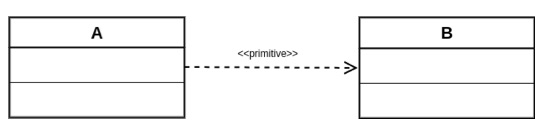
\includegraphics[scale=0.4]{Immagini/UML/Dipendenza} \\
			\captionof{figure}{Dipendenza fra classi}
		\end{center}
		\item \textbf{Associazione:} la classe A contiene dei campi dati o delle istanze di un'altra classe B. Le molteplicità possibili sono:
		\begin{itemize}
			\item \textbf{1:} A possiede un'istanza di B;
			\item \textbf{0..1:} A possiede 0 o 1 istanze di B;
			\item \textbf{0..*:} A possiede 0 o più istanze di B;
			\item \textbf{*:} A possiede più istanze di B.
		\end{itemize}
		\begin{center}
			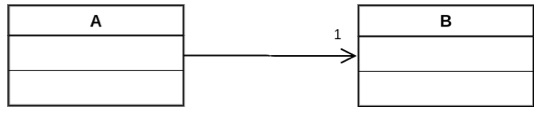
\includegraphics[scale=0.4]{Immagini/UML/Associazione} \\
			\captionof{figure}{Associazione fra classi}
		\end{center}
		\item \textbf{Aggregazione:} la classe A possiede un riferimento ad un oggetto di un'altra classe B che può essere condiviso, l'aggregato B non ha senso di esistere senza l'aggregante A;
		\begin{center}
			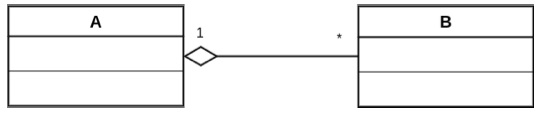
\includegraphics[scale=0.4]{Immagini/UML/Aggregazione}\\
			\captionof{figure}{Aggregazione fra classi}
		\end{center}
		\item \textbf{Composizione:} la classe A possiede un oggetto di un'altra classe B, solo l'oggetto intero può creare e distruggere le sue parti;
		\begin{center}
			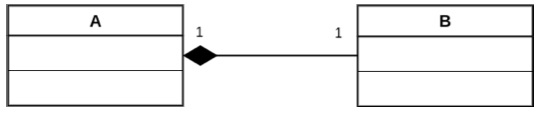
\includegraphics[scale=0.4]{Immagini/UML/Composizione} \\
			\captionof{figure}{Composizione fra classi}
		\end{center}
		\item \textbf{Generalizzazione:} la classe A generalizza un'altra classe B se ogni oggetto di B è anche un oggetto di A;
		\item \textbf{Subtyping:}  la classe A implementa l'interfaccia B. 
		\begin{center}
				\begin{minipage}{0.4\textwidth}
					\begin{center}
						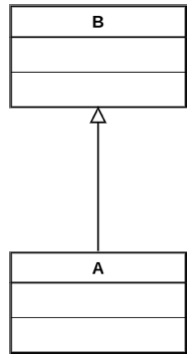
\includegraphics[scale=0.4]{Immagini/UML/Generalizzazione}\\
						\captionof{figure}{Generalizzazione fra classi}
					\end{center}
			\end{minipage}
			\begin{minipage}{0.5\textwidth}
				\begin{center}
						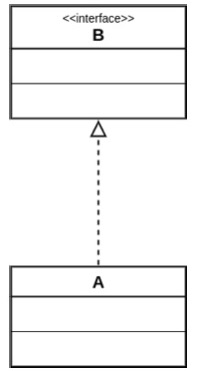
\includegraphics[scale=0.385]{Immagini/UML/Subtyping}\\
					\captionof{figure}{Subtyping fra classi}
				\end{center}
			\end{minipage}
		\end{center}	
	\end{itemize}

\paragraph*{Diagrammi dei package}
Un package rappresenta un raggruppamento di un numero arbitrario di elementi \textit{UML} in una unità di livello più alto, può quindi contenere classi (anche astratte), un altro package e interfacce. Ogni elemento di un package, identificativo di un \glo{namespace}, può avere visibilità pubblica(+) o privata(-) e deve avere un nome completamente qualificato secondo lo schema: 
\begin{center}
	\textbf{package::package::...::classe}
\end{center}
I diagrammi dei package documentano le dipendenze tra le classi che dovrebbero seguire tutte la stessa direzione evitando le dipendenze circolari.

\paragraph*{Diagrammi delle attività}
Questi diagrammi descrivono la logica procedurale e i processi di business, aiutando a descrivere gli aspetti dinamici dei casi d'uso. \\
Gli elementi di un diagramma di attività sono:
\begin{itemize}
	\item \textbf{Token:} vengono prodotti e consumati durante l'esecuzione;
	\item \textbf{Nodo iniziale:} rappresenta il punto d'inizio dell'esecuzione dell'attività, genera token;
	\item \textbf{Nodo di fine flusso:} rappresenta un punto di terminazione di un percorso di esecuzione, l'attività può continuare su altri percorsi;
	\item \textbf{Nodo finale:} rappresenta il punto di terminazione dell'esecuzione dell'attività, consuma token;
	\begin{center}
		\begin{minipage}{0.3\textwidth}
			\centering
			
\includegraphics[scale=0.2]{Immagini/UML/NodoIniziale}
			\captionof{figure}{Nodo iniziale}
		\end{minipage}
		\begin{minipage}{0.3\textwidth}
			\centering
			
\includegraphics[scale=0.2]{Immagini/UML/NodoFineFlusso}
			\captionof{figure}{Nodo fine flusso}
		\end{minipage}
		\begin{minipage}{0.3\textwidth}
			\centering
			
\includegraphics[scale=0.19]{Immagini/UML/NodoFinale}
			\captionof{figure}{Nodo finale}
		\end{minipage}
	\end{center}
	\item \textbf{Activity:} rappresenta un'azione all'interno dell'attività, identificata da una breve descrizione;
	\item \textbf{Subactivity:} rappresenta una sotto-attività utilizzata per descrivere un'azione che ne comprende altre al suo interno, il suo diagramma viene fornito separatamente. Ogni sotto-attività è composta dall'input, dall'output e dalle azioni contenute.
	\begin{center}
		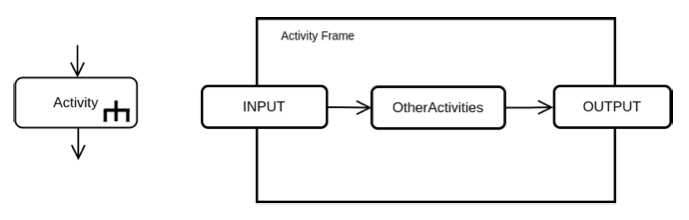
\includegraphics[scale=0.4]{Immagini/UML/Sottoattivita}
		\captionof{figure}{Attività che presenta una sotto-attività}
	\end{center}
	\item \textbf{Pin:} rappresenta un parametro prodotto o consumato da un'azione, va indicato il formato del parametro;
	\begin{center}
		\centering
		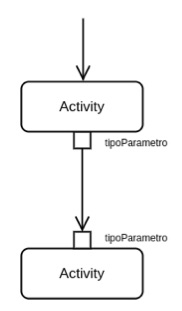
\includegraphics[scale=0.4]{Immagini/UML/Pin}
		\captionof{figure}{Attività che presenta un pin}
	\end{center}
	\item \textbf{Fork:} rappresenta un punto d'inizio di un elaborazione parallela all'interno dell'attività, produce un token per ogni processo;
	\item \textbf{Join:} rappresenta un punto di sincronizzazione tra i processi paralleli, consuma i token in ingresso e ne genera solo uno;
	\item \textbf{Branch:} rappresenta un punto di decisione tra i possibili percorsi di esecuzione in base alla guardia associata;
	\item \textbf{Merge:} rappresenta un punto di unione dei diversi percorsi di esecuzione (non paralleli) generati in seguito ad un branch, il token viene solo instradato;
	\begin{center}
		\begin{minipage}{0.4\textwidth}
			\centering
			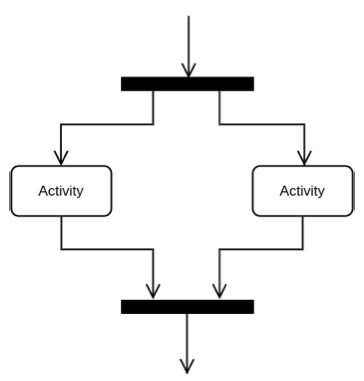
\includegraphics[scale=0.453]{Immagini/UML/ForkJoin}
			\captionof{figure}{Fork e Join}
		\end{minipage}
		\begin{minipage}{0.4\textwidth}
			\centering
			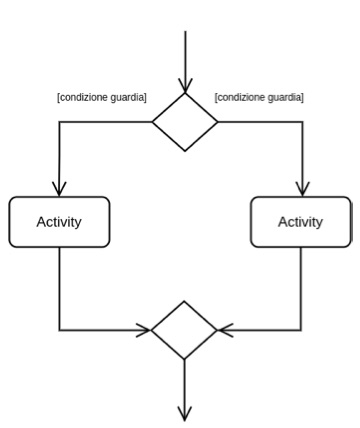
\includegraphics[scale=0.4]{Immagini/UML/BranchMerge}
			\captionof{figure}{Branch e Merge}
		\end{minipage}
	\end{center}
	\item \textbf{Segnale:} rappresenta un evento esterno, generato in modo non bloccante e catturato in modo bloccante, all'interno dell'attività;
	\begin{center}
		\centering
		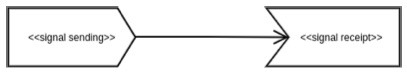
\includegraphics[scale=0.5]{Immagini/UML/Segnali}
		\captionof{figure}{Segnali in un diagramma attività}
	\end{center}
	\item \textbf{Timeout:} rappresenta un'attesa bloccante all'interno dell'attività, di cui deve essere specificata la durata e l'unità di misura, o un evento ripetuto nel tempo;
	\begin{center}
		\centering
		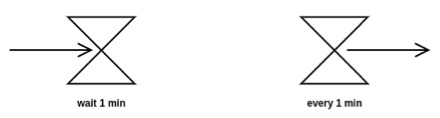
\includegraphics[scale=0.5]{Immagini/UML/Timeout}
		\captionof{figure}{Timeout in un diagramma attività}
\end{center}
	\item \textbf{Swimlane:} fornisce una responsabilità all'esecuzione delle azioni all'interno di un'attività.
\end{itemize}

\paragraph*{Diagrammi di sequenza}
I diagrammi di sequenza descrivono la collaborazione di un gruppo di oggetti che devono implementare collettivamente un comportamento.
Gli elementi utilizzati in questi diagrammi sono i seguenti:
\begin{itemize}
	\item \textbf{Partecipante:} entità che detiene il flusso di esecuzione del caso d'uso, è composto di due parti:
	\begin{itemize}
		\item \textbf{Nome:} nome dell'entità partecipante;
		\item \textbf{Barra di attivazione:} indica il periodo di tempo durante il quale il partecipante è attivo;
	\end{itemize}
	\item \textbf{Messaggio:} rappresenta dati e operazioni scambiati tra partecipanti, può essere di una delle seguenti tipologie:
	\begin{itemize}
		\item \textbf{Sincrono:} il chiamante rimane in attesa della risposta;
		\item \glo{\textbf{Asincrono:}} il chiamante non attende la risposta; 
		\item \textbf{Ritorno:} messaggio di ritorno riferito ad un precedente messaggio di chiamata;
		\item \textbf{Creazione:} messaggio di creazione di un nuovo partecipante da parte del partecipante chiamante;
		\item \textbf{Distruzione:} messaggio di distruzione di un partecipante da parte del partecipante chiamante.
	\end{itemize}
\end{itemize}
\begin{center}
	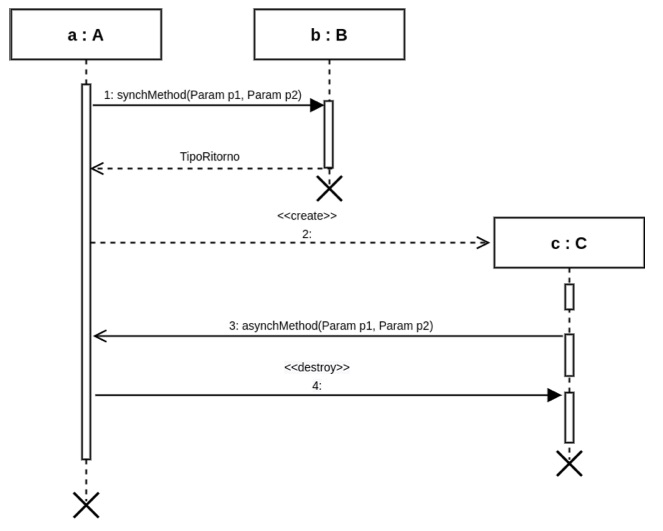
\includegraphics[scale=0.5]{Immagini/UML/DSequenza} \\
	\captionof{figure}{Esempio di diagramma di sequenza}
\end{center}

\paragraph*{Diagrammi dei casi d'uso}
Un caso d'uso è un'insieme di scenari (sequenze di azioni) che hanno in comune uno scopo finale per un utente. I diagrammi dei casi d'uso sono una rappresentazione grafica dei casi d'uso analizzati nel documento di \AdRv. Vengono messi in evidenza:
\begin{itemize}
	\item \textbf{Attori:} rappresentano tutto ciò che è esterno al sistema e interagisce con esso;
	\item \textbf{Use Case:} rappresentano le attività associate al sistema.
\end{itemize}
Le eventuali relazioni tra gli Use Case del sistema rappresentate in questi diagrammi sono: 
\begin{itemize}
	\item \textbf{Inclusione:} si ha quando vi sono funzionalità comuni fra più casi d'uso, lo use case B è incondizionatamente incluso nell'esecuzione dello use case A;
	\begin{center}
		\centering
		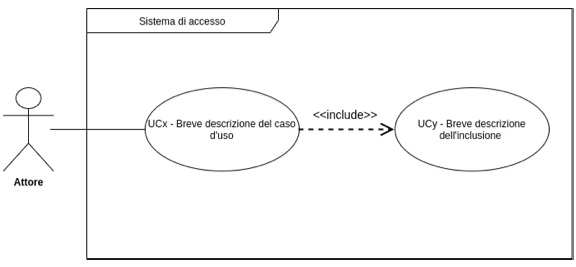
\includegraphics[scale=0.4]{Immagini/UML/Inclusione}
		\captionof{figure}{Inclusione casi d'uso}
	\end{center}
	\item \textbf{Estensione:} si ha se ogni istanza dello use case A esegue lo use case B in modo condizionato, l'esecuzione di B interrompe A;
	\begin{center}
		\centering
		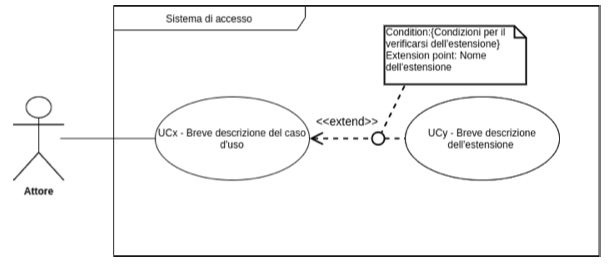
\includegraphics[scale=0.4]{Immagini/UML/Estensione}
		\captionof{figure}{Estensione casi d'uso}
	\end{center}
	\item \textbf{Generalizzazione:} si ha quando si vogliono aggiungere o modificare caratteristiche base, in particolare si ha che:
	\begin{itemize}
		\item L'attore A è generalizzazione dell'attore B se B condivide almeno le funzionalità di A;
		\item I casi d'uso figli aggiungono funzionalità rispetto ai padri o ne modificano il comportamento.
	\end{itemize}
	\begin{center}
		\begin{minipage}{0.4\textwidth}
			\centering
			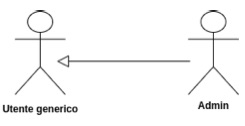
\includegraphics[scale=0.4]{Immagini/UML/GeneralizzazioneAttori}
			\captionof{figure}{Generalizzazione tra attori}
		\end{minipage}
		\begin{minipage}{0.5\textwidth}
			\centering
			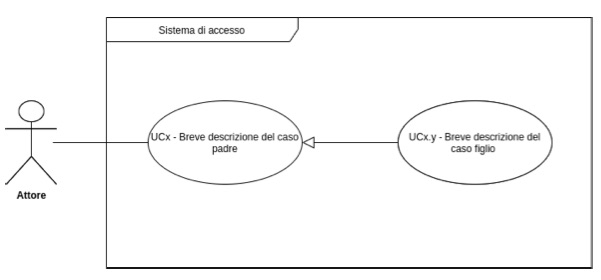
\includegraphics[scale=0.4]{Immagini/UML/GeneralizzazioneUC}
			\captionof{figure}{Generalizzazione Casi d'uso}
	\end{minipage}
	\end{center}
\end{itemize} 




\subsubsection{Codifica software}
\myparagraph{Scopo dell'attività} 
L'attività di codifica svolta dai \textit{Programmatori} ha lo scopo di trasformare in codice quanto previsto dall'attività di progettazione svolta dai \textit{Progettisti}, procedendo all'effettiva realizzazione del prodotto software richiesto.

\myparagraph{Descrizione della sezione}
La sezione tratta le norme da seguire per ogni linguaggio di programmazione utilizzato durante lo svolgimento del progetto.

\myparagraph{Aspettative}\label{AspettativeCodifica}Con le norme individuate il gruppo si aspetta la realizzazione di codice uniforme. Per assicurare il raggiungimento degli obiettivi di qualità previsti dal \PdQ\ il gruppo intende:
\begin{itemize}
	\item Utilizzare i linguaggi sfruttando adeguatamente le loro capacità;
	\item Ridurre il numero di righe di codice che possono causare errori;
	\item Redarre il codice affinché si chiaro nel tempo e facilmente comprensibile anche da altri programmatori.
\end{itemize}

\myparagraph{Qualità della codifica}
La codifica è di qualità se: 
\begin{itemize}
	\item Il codice è facilmente leggibile;
	\item I costrutti del linguaggio sono utilizzati in modo chiaro e coerente;
	\item La compilazione non presenta errori fatali o potenziali.
\end{itemize}
Queste caratteristiche sono in grado di agevolare manutenzione, verifica e validazione e di conseguenza migliorare la qualità di prodotto.

\myparagraph{Convenzioni generiche}\label{CodificaConvenzioni}
Vengono di seguito riportate le norme generiche stabilite per la codifica.
\paragraph*{Intestazione}
I file sorgenti consegnati presentano la seguente intestazione inserita in un blocco di commento.
\paragraph*{Nomenclatura}
Tutte le classi, i metodi, le variabili devono avere un nome univoco, esplicativo e scritto in lingua inglese, in particolare:
\begin{itemize}
	\item Per i nomi di cartelle, file e classi viene seguita la convenzione \textbf{CamelCase};
	\item I nomi di variabili e metodi hanno iniziale minuscola, se composti da più parole la prima lettera delle parole successive alla prima è maiuscola;
	\item Le costanti vengono scritte in maiuscolo.
\end{itemize}
\paragraph*{Parentesi}
I blocchi di codice vanno inseriti tra parentesi graffe, anche se il blocco è vuoto o costituito da una sola riga di codice.
\paragraph*{Verbosità}
Una riga di codice deve essere lunga al massimo 140 caratteri. Se possibile è desiderabile definire metodi brevi evitando la ricorsione.

\myparagraph{Metriche}\label{MCodifica}Di seguito vengono presentate le metriche utilizzate per garantire il controllo sulla qualità. Per una descrizione sullo standard di riferimento e un elenco completo di tutte le metriche applicate si rimanda alla sezione \S\ref{9126} dell'appendice. 
\begin{itemize}
	\item\textbf{MPDS01: Completezza dell'implementazione}\hypertarget{MCImplementazione} \\
	L'indice stabilisce la completezza del prodotto software realizzato nel momento in cui viene calcolato rispetto a tutti i requisiti previsti dall'\AdRv{1.0.0}.\\
	Viene calcolato nel seguente modo:
	\begin{center}
		\textbf{CI=\(1-\frac{FNI}{FI}\)*100}
	\end{center}
	dove:
	\begin{itemize}
		\item \textbf{FNI} indica il numero di funzionalità non implementate;
		\item \textbf{FI} indica il numero di funzionalità implementate.
	\end{itemize}
\item\textbf{MPDS02: Densità errori} \hypertarget{MErrori}\\
Rappresenta la percentuale di righe di codice che possono causare errori.\\
Viene calcolato nel seguente modo:
\begin{center}
	\textbf{DE=\(\frac{RB}{RTOT}\)*100}
\end{center}
dove:
\begin{itemize}
	\item \textbf{RB} indica il numero di linee di codice che possono causare imprevisti o comportamenti diversi da quelli desiderati;
	\item \textbf{RTOT} indica il numero di linee di codice totali.
\end{itemize}

\item\textbf{MPDS07: Facilità di comprensione} \hypertarget{MFComprensione}\\
Il valore indica la facilità di comprensione del codice in base al numero di righe di commento presenti.\\
Viene calcolato nel seguente modo:
\begin{center}
	\textbf{FC=\(\frac{LCOM}{LCOD}\)*100}
\end{center}
dove
\begin{itemize}
	\item \textbf{LCOM} indica il numero di linee di commento;
	\item \textbf{LCOD} indica il numero di linee di codice.
\end{itemize}

\item\textbf{MPDS08: Semplicità delle funzioni}\hypertarget{MSFunzioni}\\
Il valore stabilisce la semplicità di un metodo basandosi sul numero di parametri a lui necessari.

\item\textbf{MPDS09: Semplicità delle classi}\hypertarget{MSClassi}\\
Il valore stabilisce la semplicità di una classe basandosi sul numero di metodi al suo interno.
\end{itemize}

\subsubsection{Strumenti}
\newpage

\newpage

\section{Processi di Supporto}
\subsection{Descrizione}
I Processi di Supporto comprendono tutti i processi che nell'eseguire una specifica funzione forniscono supporto ad un altro processo che li esegue, contribuendo al successo e alla qualit\'a di un progetto. \\
I Processi di Supporto analizzati in questa sezione sono:
\begin{itemize}
	\item \textbf{Documentazione;}
	\item \textbf{Gestione della Configurazione;}
	\item \textbf{Gestione della Qualit\'a;}
	\item \textbf{Verifica;}
	\item \textbf{Validazione;}
	\item \textbf{Gestione dei Cambiamenti;}
\end{itemize}

\subsection{Documentazione}
\subsubsection{Scopo dell'attività} \label{PSup_Documentazione_Scopo}
Quando si realizza un progetto è di fondamentale importanza documentare processi e attività significative per lo sviluppo dello stesso. \\
La Documentazione permette di:
\begin{itemize}
	\item Disciplinare ciò che verrà fatto durante il ciclo di vita del software;
	\item Garantire che tutte le informazioni d'interesse siano facilmente accessibili agli stakeholders;
	\item Assicurare che quanto previsto dalla Documentazione sia rispettato per garantire la qualità attesa.
\end{itemize}

\subsubsection{Descrizione della sezione} 
La sezione comprende le norme relative alla documentazione associata al progetto che tutti i componenti devono seguire nella redazione dei documenti di loro competenza.

\subsubsection{Aspettative}
L'obiettivo del gruppo è di ottenere dei prodotti documentali coerenti e validi dal punto di vista tipografico e formale.
I documenti prodotti dal gruppo devono:
\begin{itemize}
	\item Essere facilmente aggiornabili e modificabili;
	\item Contenere solo ciò che è essenziale;
	\item Essere facili da leggere.
\end{itemize}

\subsubsection{Ciclo di vita di un documento}\label{CicloDocumentazione}
Tutti i documenti prodotti sono sottoposti a queste attività:
\begin{itemize}
	\item \textbf{Creazione: }il documento viene creato secondo il template presente nella repository;
	\item \textbf{Stesura: }il documento viene redatto dai componenti incaricati, tutti i documenti devono contenere:
	\begin{itemize}
		\item Registro delle Modifiche;
		\item Indice dei Contenuti;
	\end{itemize}
	\item \textbf{Revisione: }le sezioni del documento vengono regolarmente revisionate da uno o più componenti del gruppo diversi dai redattori delle stesse;
	\item \textbf{Approvazione: }il \Responsabile\ stabilisce la validità del documento che ora può essere rilasciato. 
\end{itemize}

\subsubsection{Classificazione dei documenti}\label{ClassificazioneDocumenti}
I documenti vengo suddivisi in:
\begin{itemize}
	\item \textbf{Documenti Pubblici: }comprendono i documenti di interesse per il gruppo, il proponente e il committente. 
	Sono documenti pubblici:
	\begin{itemize}
		\item \textbf{Glossario: }elenco ordinato di termini utilizzati dal gruppo nei loro documenti e che possono presentare ambiguità nel loro significato;
		\item \textbf{Studio di Fattibilità: }analisi dei capitolati proposti, con le valutazioni da parte dei membri del gruppo;
		\item \textbf{Piano di Progetto: }espone la pianificazione delle attività di progetto e relative previsioni rispetto a impiego orario dei membri, preventivo spese e consuntivi di periodo;
		\item \textbf{Piano di Qualifica: }presenta i criteri di valutazione della qualità utilizzati dal gruppo;
		\item \textbf{Analisi dei Requisiti: }contiene tutti i requisiti e le caratteristiche del prodotto finale individuati dal gruppo.
	\end{itemize}
	\item Documenti Interni: comprendono i documenti di interesse principalmente per i componenti del gruppo.
	Sono documenti interni:
	\begin{itemize}
		\item \textbf{Norme di Progetto:} raccolta delle norme stabilite dal gruppo che tutti i componenti devono seguire durante la realizzazione del progetto;
		\item \textbf{Verbali:} si suddividono a loro volta in:
		\begin{itemize}
			\item \textbf{Interni:} contengono un resoconto sintetico relativo alle riunioni svolte dal gruppo;
			\item \textbf{Esterni:} contengono un resoconto relativo alle riunioni del gruppo con il proponente e/o i commitenti.
		\end{itemize}
	\end{itemize}
\end{itemize}

\subsubsection{Nomenclatura dei documenti} \label{NomenclaturaDoc}
Tutti i documenti ad eccezione dei Verbali seguiranno il seguente schema per la nomenclatura:

\begin{center}
	\textbf{[NomeDocumento]\_v[X].[Y].[Z]}
\end{center}
dove:
\begin{itemize}
	\item \textbf{[NomeDocumento]} corrisponde al nome ufficiale del documento, non deve presentare spazi e viene utilizzata la notazione \textit{CamelCase}.
	\item \textbf{v[X].[Y].[Z]} dove v sta per "versione" e X, Y, Z rispettano quanto descritto nella sezione \S\ref{Versionamento}
\end{itemize}

Per quanto riguarda la nomenclatura dei Verbali si segue il seguente schema:
\begin{center}
	\textbf{V[I/E]\_[YYYY]\_[MM]\_[DD]}
\end{center}
dove:
\begin{itemize}
	\item \textbf{V: } indica che il documento è un Verbale;
	\item \textbf{[I/E]: } indica se il Verbale è interno o esterno;
	\item \textbf{[YYYY]\_[MM]\_[DD]: } indica la data in cui si è svolto l'incontro indicata come anno\_mese\_giorno.
\end{itemize}

\subsubsection{Directory dei documenti}
Ogni documento viene inserito in una directory il cui nome coincide con il NomeDocumento dello stesso, posizionata a sua volta secondo la tipologia del documento contenuto nella directory \textbf{DocumentiInterni} o \textbf{DocumentiPubblici}.

\subsubsection{Struttura dei documenti}\label{StrutturaDocumenti}
Tutti i documenti contengono prima delle pagine con il contenuto previsto:
\begin{itemize}
\item \textbf{Frontespizio}:
La prima pagina di ogni documento comprende in sequenza i seguenti elementi:
\begin{itemize}
	\item \textbf{Logo del gruppo; }
	\item \textbf{Nome del documento;}
	\item \textbf{Nome del gruppo e del Progetto;}
	\item \textbf{Email del gruppo;}
	\item \textbf{Informazioni sul documento}, che includono:
		\begin{itemize}
			\item \textbf{Versione;}
			\item \textbf{Approvatore;}
			\item \textbf{Redattori;}
			\item \textbf{Verificatori;}
			\item \textbf{Uso} se interno o pubblico;
			\item \textbf{Distribuzione}, cioè i destinatari del documento.
		\end{itemize}
	\item \textbf{Descrizione} breve del contenuto del documento.
\end{itemize}

\item\textbf{Registro delle Modifiche}
Sotto forma di tabella viene presentato un registro delle modifiche contenente le modifiche effettuate al documento durante il suo ciclo di vita e le varie verifiche effettuate.\\
Ciascuna voce della tabella riporta:
\begin{itemize}
	\item \textbf{Versione} del documento dopo la modifica/verifica;
	\item \textbf{Data} della modifica/verifica;
	\item \textbf{Nominativo} del componente che ha effettuato la modifica/verifica;
	\item \textbf{Ruolo} del componente che ha effettuato la modifica/verifica;
	\item \textbf{Descrizione} della modifica/verifica effettuata.
\end{itemize}
Per garantire la consistenza del Registro delle Modifiche le sezioni sono etichettate con il comando \LaTeX\ \textit{label}, le sezioni che vengono eliminate sono indicate con il loro titolo.

\item\textbf{Indice}
Dopo il registro delle modifiche viene inserito un indice dei contenuti utile a chi utilizza il documento per orientarsi velocemente all'interno dello stesso.

\item\textbf{Corpo dei documenti}
Dopo l'indice dei contenuti è presente il corpo del documento. Gli argomenti sono divisi in sezioni e sottosezioni raggruppati in modo coerente e coeso. \\
Il corpo dei Verbali deve contenere le seguenti sezioni:
\begin{itemize}
	\item \textbf{Informazioni Generali}, che includono:
		\begin{itemize}
			\item \textbf{Luogo} in cui si è svolta la riunione;
			\item \textbf{Data} in cui si è svolta la riunione;
			\item \textbf{Ora}, comprendente orario di inzio e di fine;
			\item \textbf{Partecipanti}, membri del gruppo ed eventualmente committenti e/o proponente;
			\item \textbf{Segretario}, componente del gruppo che ha redatto il verbale.
		\end{itemize}
	\item \textbf{Ordine del giorno: }argomenti principali di cui si è trattato.
	\item \textbf{Resoconto: }per ogni argomento trattato è presente una breve descrizione della discussione avvenuta;
	\item \textbf{Registro delle decisioni:} vengono presentate sotto forma di elenco le decisioni prese dal gruppo.
\end{itemize}
\end{itemize}

\subsubsection{Formattazione e norme tipografiche}
\myparagraph{Template}
Il gruppo utilizza per la stesura dei documenti il linguaggio \LaTeX. Al fine di mantenere una coerenza nella formattazione dei documenti vengono utilizzati due template permettendo così l'automatizzazione delle scelte tipografiche. \\
I template utilizzati sono:
\begin{itemize}
	\item \textbf{StileLettera: }template esclusivamente per le Lettere di Presentazione;
	\item \textbf{StileTemplate: }template per tutti i restanti documenti.
\end{itemize}

\myparagraph{Termini di glossario}
I termini il cui significato potrebbe essere ambiguo sono individuati con un apice \ap{G} alla fine della parola, salvo che il suo significato non venga subito spiegato. Tutti i termini da glossario sono stati inseriti nel documento \Glossariov.

\myparagraph{Stile del testo}
Gli stili di testo adottati nei documenti sono:
\begin{itemize}
	\item \textbf{grassetto:} per titoli, sottotitoli, nome degli oggetti negli elenchi puntati, termini importanti secondo il \textit{Redattore};
	\item \textbf{corsivo:} per i nomi propri, nomi dei ruoli, nome del progetto, nome dei documenti, nomi delle tecnologie, degli strumenti, delle formule matematiche, termini specifici e citazioni.
	\item \textbf{maiuscolo:} per i nomi dei file, delle directory e dei processi (convenzione \textit{CamelCase}).	
\end{itemize}

\myparagraph{Formattazione di date e orari}
Per l'indicazione delle date e degli orari si segue quanto sancito dallo standard ISO \glo{8601}. \\
Le date vengono indicate secondo il seguente formato:
\begin{center}
	\textbf{[YYYY]\_[MM]\_[DD]} 
\end{center}
dove:
\begin{itemize}
	\item \textbf{[YYYY]} corrisponde all'anno;
	\item \textbf{[MM]} corrisponde al mese;
	\item \textbf{[DD]} corrisponde al giorno.
\end{itemize}
Gli orari vengono indicati secondo il seguente formato:
\begin{center}
	\textbf{[HH]:[MM]} 
\end{center}
dove:
\begin{itemize}
	\item \textbf{[HH]} rappresenta l'ora;
	\item \textbf{[MM]} rappresenta i minuti;
\end{itemize}

\myparagraph{Formattazione elementi grafici}
La sezione definisce le norme per gli elementi grafici all'interno dei documenti.
\begin{itemize}
\item\textbf{Immagini}
Le figure presenti nei documenti vanno centrate rispetto al testo e accompagnate da una didascalia coerente.
\item\textbf{Grafici UML}
I grafici in linguaggio \glo{UML} sono inseriti come immagini.
\item\textbf{Tabelle}
Le tabelle vanno accompagnate da una didascalia opportuna.\\
Nella didascalia viene indicato l'identificativo 
\begin{center}
	\textbf{Tabella [X]} 
\end{center}
dove [X] inidica il numero assoluto della tabella all'interno del documento; segue poi il testo della didascalia.
A questa prassi fanno eccezione le tabelle del registro delle modifiche.
\end{itemize}

\subsubsection{Strumenti} \label{Documentazione_Strumenti}
Gli strumenti utilizzati per la stesura dei documenti sono:
\begin{itemize}
	\item Linguaggio \LaTeX
\end{itemize}

\subsubsection{Metriche} 
\subsubsection{Verifica ortografica} 

\newpage
\subsection{Gestione della configurazione}
\subsubsection{Scopo dell'attività} \label{PSup_GestioneConf_Scopo}
La gestione della configurazione ha lo scopo di gestire ordinatamente e sistematicamente la produzione dei documenti e del codice.

\subsubsection{Descrizione della sezione} 
La sezione presenta le norme che il gruppo intende seguire per il controllo della documentazione e del codice.

\subsubsection{Aspettative}
Con queste norme il gruppo intende assicurare una corretta gestione dei documenti e del codice rendendo sistematica la loro produzione e garantendo la chiara individuazione delle versioni prodotte.

\subsubsection{Identificazione di configurazione}
Ogni \glo{configuration item} ha un'identità unica che ne consente la chiara individuazione. Per una trattazione precisa si rimanda alla sezione \S\ref{NomenclaturaDoc}.

\subsubsection{Controllo di baseline}
Per garantire riproducibilità e tracciabilità viene definita una successione di \glo{baseline} associate a una serie di \glo{milestone} specifiche per obiettivi di avanzamento e coerenti con la strategia di progetto. Data l'importanza di controllare lo svolgimento del progetto il numero delle milestone sarà superiore al numero delle revisioni.

\subsubsection{Controllo di versione}\label{Versionamento}
\myparagraph{Codice di versione per documenti e software}
Il codice di una versione è formato: 
\begin{center}
	\textbf{[X].[Y]}
\end{center}
dove 
\begin{itemize}
	\item \textbf{[X]} corrisponde ad una versione del documento approvata dal \Responsabile\ e pronta al rilascio, la numerazione parte da 0;
	\item \textbf{[Y]} corrisponde ad una versione del documento verificata in tutte le sue parti, inizia da 0 e riparte da questo valore ad ogni incremento di X;
\end{itemize}
Il controllo di versione si appoggia su un repository creato in \glo{Github} la cui struttura viene spiegata nella sezione seguente.

\subsubsection{Struttura della repository}\label{StrutturaRepo}
La repository del gruppo \Gruppo\ è accessibile all'indirizzo
\begin{center}
	\textbf{https://github.com/NotOnlyStudents}
\end{center}
L'utilizzo di questo strumento permette a ciascun componente di lavorare sui \glo{configuration items} senza rischio di sovrascritture consentendo allo stesso tempo di controllare l'andamento del lavoro. 
All'interno del repository viene divisa la documentazione dal codice software.
\myparagraph{Repository per la documentazione}\label{RepoDoc}
Il repository per la documentazione è composto da diversi \textbf{branch}:
\begin{itemize}
	\item \textbf{master} su cui vengono riportati i documenti approvati dal \Responsabile\ e pronti nella loro versione definitiva ad essere presentati;
	\item \textbf{develop} ramo in cui vengono inserite la versioni dei documenti verificati ma non ancora approvati;
	\item rami dedicati ai singoli documenti in sviluppo non verificati.
\end{itemize}
All'interno del repository troviamo le cartelle così organizzate:
\begin{itemize}
	\item \textbf{Immagini}: contiene le immagini utilizzate all'interno dei documenti;
	\item \textbf{Utilita}: contiene file di utilità per la produzione di tutti i documenti;
	\item \textbf{DocumentiInterni}: contiene le cartelle dei documenti di interesse per il gruppo e marginale per proponente e committenti;
	\item \textbf{DocumentiPubblici}: contiene le cartelle dei documenti di interesse per il gruppo, per il proponente e per i committenti.
\end{itemize}
\myparagraph{Modifiche al repository}\label{ModificaRepo}
Nel caso fosse necessario modificare file all'interno del ramo master è necessaria una \textbf{pull request} con conseguente approvazione da almeno un altro elemento del gruppo.
\newpage
\subsection{Gestione della qualità}
\subsubsection{Scopo dell'attività} 
L'attività ha lo scopo di assicurare al proponente che il prodotto realizzato soddisfi i requisiti e la qualità previsti e stabiliti con il proponente.
\subsubsection{Descrizione della sezione} 
La sezione presenta il processo utilizzato dal gruppo per gestire il \glo{Sistema Qualità}, indicando procedure e strumenti utili che i componenti devono seguire.
\subsubsection{Aspettative}
Il gruppo si aspetta da questo processo di conseguire la qualità del prodotto prevista secondo le aspettative del proponente attraverso un'azione preventiva. Il documento \PdQ individua quanto stabilito indicando gli obiettivi di qualità da raggiungere e le \glo{metriche} da utilizzare per la valutazione della qualità.
\subsubsection{Istanziazione di un processo}
Perseguendo la qualità attraverso un'azione preventiva, il gruppo deve compiere le proprie scelte considerando le caratteristiche di qualità ricercate. 
Le seguenti norme devono essere considerate con l'istanziazione di ogni processo:
\begin{itemize}
	\item Ogni processo deve puntare a perseguire un unico obiettivo;
	\item Ad ogni istanziazione di un processo devono essere analizzati i rischi connessi e prevedendo una pianificazione del lavoro per il loro contrasto;
	\item Ad ogni istanziazione di un processo le risorse vengono assegnate considerando gli altri processi già in esecuzione;
	\item Ogni processo deve avere una durata definita.
\end{itemize}
\subsubsection{Svolgimento di un processo}
Durante lo svolgimento di un processo, le attività vengono svolte perseguendo il raggiungimento degli obiettivi individuati all'interno del \PdQv{} e le seguenti caratteristiche di qualità:
\begin{itemize}
	\item \textbf{Qualità di prodotto}: 
	\begin{itemize}
		\item \textbf{Adeguatezza Funzionale};
		\item \textbf{Efficienza Prestazionale};
		\item \textbf{Usabilità};
		\item \textbf{Affidabilità};
		\item \textbf{Sicurezza};
		\item \textbf{Manutenibilità};
	\end{itemize}
	\item \textbf{Qualità in uso}: 
	\begin{itemize}
		\item \textbf{Efficacia};
		\item \textbf{Efficienza};
		\item \textbf{Soddisfazione};
		\item \textbf{Mitigazione dei rischi};
		\item \textbf{Copertura dei requisiti};
	\end{itemize}
\end{itemize}
\subsubsection{Classificazione degli obiettivi}
Gli obiettivi di qualità presenti nel \PdQv{} vengono classificate secondo il seguente formato:
\begin{center}
	\textbf{O[Categoria][D/S][X]}
\end{center}
dove 
\begin{itemize}
	\item \textbf{O} indica che si tratta di un obiettivo di qualità;
	\item \textbf{Categoria} può assumere i seguenti valori:
	\begin{itemize}
		\item \textbf{PR:} l'obiettivo riguarda un processo;
		\item \textbf{PD:} l'obiettivo riguarda un prodotto.
	\end{itemize}
	\item \textbf{D/S} indicano rispettivamente se l'obiettivo riguarda un documento o un prodotto software, è presente solo per gli obiettivi relativi ai prodotti;
	\item \textbf{X} è un numero progressivo che inizia da 1.
\end{itemize}
\subsubsection{Classificazione delle metriche}
Le metriche utilizzate per la valutazione della qualità presenti nel \PdQv{} vengono classificati secondo il seguente formato:
\begin{center}
	\textbf{M[Categoria][D/S][X]}
\end{center}
dove 
\begin{itemize}
	\item \textbf{M} indica che si tratta di una metrica di qualità;
	\item \textbf{Categoria} può assumere i seguenti valori:
	\begin{itemize}
		\item \textbf{PR:} la metrica riguarda un processo;
		\item \textbf{PD:} la metrica riguarda un prodotto.
	\end{itemize}
	\item \textbf{D/S} indicano rispettivamente se l'obiettivo riguarda un documento o un prodotto software,è presente solo per gli obiettivi relativi ai prodotti;
	\item \textbf{X} è un numero progressivo che inizia da 1.
\end{itemize}
\subsubsection{Metriche}
\newpage
\subsection{Verifica}\label{Verifica}
\subsubsection{Scopo dell'attività} \label{PSup_Verifica_Scopo}
L'attività di Verifica ha lo scopo di accertare che quanto eseguito durante il periodo preso in considerazione non abbia introdotto errori e quindi che quanto realizzato sia corretto e completo.
\subsubsection{Descrizione della sezione} 
La sezione descrive come avviene l'attività di verifica da parte del gruppo \Gruppo\ per la documentazione e il codice.
\subsubsection{Aspettative}
Utilizzando le norme presenti il gruppo si aspetta di ottimizzare e uniformare il processo di verifica. 
L'attività di Verifica viene attuata attraverso l'Analisi Statica e l'Analisi Dinamica. 
\subsubsection{Analisi Statica}
L'Analisi Statica studia la documentazione e il codice accertando che siano conformi alle regole stabilite, non vi siano difetti e presentino le proprietà desiderate.
Il \textit{Verificatore} seguirà uno dei seguenti metodi:
\begin{itemize}
	\item \textbf{Walkthrough:} procede ad una lettura critica dell'intero prodotto in esame alla ricerca di difetti;
	\item \textbf{Inspection:} procede ad una lettura critica di una parte prodotto in esame, focalizzando la ricerca su problemi che si presentano più frequentemente indicati nella Lista di Controllo all'interno del \PdQv{}.
\end{itemize}

\myparagraph{Verifica della documentazione}\label{VerificaDocumentazione}
Il \textbf{Verificatore} incaricato procede nel seguente modo:
\begin{itemize}
	\item Se non ancora creata, crea l'issue in GitHub;
	\item Sposta l'issue in "IN PROGRESS";
	\item Rilegge il documento secondo uno dei due metodi previsti, nel caso di Inspection valuta l'aggiornamento della Lista di Controllo;
	\item Se riscontra problemi logici,si accorda con il redattore del documento per la correzione. 
	\item Procede al controllo ortografico automatico utilizzando \textit{Aspell};
	\item Sposta l'issue in "DONE".
\end{itemize}

\myparagraph{Verifica del codice}\label{VerificaCodice}
Il \textit{Verificatore} incaricato procede nel seguente modo:
\begin{itemize}
	\item Se non ancora creata, crea l'issue in GitHub;
	\item Sposta l'issue in "IN PROGRESS";
	\item Rilegge il codice secondo uno dei due metodi previsti al fine di:
	\begin{itemize}
		\item Accertare che il codice esegua nella sequenza specificata e sia ben strutturato;
		\item Localizzare codice non raggiungibile;
		\item Identificare parti di codice che possano non terminare;
		\item Accertare che nessun cammino acceda a variabili prive di valore;
		\item Rilevare anomalie;
		\item Provare la correttezza del codice sorgente rispetto ai requisiti;
		\item Assicurare che sia stato seguito quanto scritto nelle \NdPv{}\ nella sezione \S\ref{CodificaConvenzioni}.
	\end{itemize}
	 Nel caso di Inspection valuta l'aggiornamento della Lista di Controllo;
	\item Se riscontra problemi, si accorda con il redattore del documento per la correzione. 
	\item Sposta l'issue in "DONE".
\end{itemize}

\subsubsection{Analisi Dinamica}
L'Analisi Dinamica procede a verificare il programma durante la sua esecuzione. Per procedere a questa attività vengono utilizzati dei test ripetibili e automatizzati con specifici:
\begin{itemize}
	\item \textbf{Ambiente di esecuzione};
	\item \textbf{Input e Output};
	\item \textbf{Procedure};
\end{itemize}

\myparagraph{Tipologia di test effettuati}\label{Tests}
I test permettono di valutare se il programma svolge i tasks per cui è stato sviluppato. Il \PdQv{}\ specifica quali e quanti test effettuare.
\paragraph*{Test d'unità}
I test d'unità consistono nell'isolare e testare la parte più piccola di software, chiamata appunto unità. Lo scopo è di valutare la logica interna del codice d'unità in modo da poterne stabilire il corretto funzionamento. 
\paragraph*{Test d'integrazione}
Applicati alle componenti della progettazione architetturale, hanno lo scopo di valutare che l'aggregazione delle parti del sistema non introduca errori nel software prodotto.
\paragraph*{Test di regressione}
Questi test sono necessari a verificare che la modifica di una parte P di S non causi errori in P, in S o in una parte in relazione con essi. Le modifiche apportate non devono pregiudicare le funzionalità già verificate. 
\paragraph*{Test di sistema}
Vengono effettuati per valutare che il prodotto soddisfi tutti i requisiti software previsti.

\myparagraph{Procedura di verifica}\label{ProceduraVerifica}
Il \textit{Verificatore} incaricato procede nel seguente modo:
\begin{itemize}
	\item Se non ancora creata, crea l'issue in GitHub;
	\item Sposta l'issue in "IN PROGRESS";
	\item Esegue tutti i test previsti;
	\item Se riscontra problemi, si accorda con il redattore del codice per la correzione. 
	\item Sposta l'issue in "DONE".
	\item Avverte i redattori incaricati ad aggiornare il \PdQv{} con i risultati ottenuti.
\end{itemize}


\subsubsection{Strumenti}

\newpage
\subsection{Validazione}\label{PSup_Validazione}
\subsubsection{Scopo dell'attività} 
La Validazione stabilisce se il prodotto soddisfi i compiti per cui è stato creato, in particolare permette di garantire che quanto richiesto e stabilito dal \Proponente\ sia soddisfatto.
\subsubsection{Descrizione della sezione} 
La sezione descrive la procedura seguita per la validazione di quanto viene prodotto durante il progetto.
\subsubsection{Aspettative}
Il gruppo si aspetta di procedere alla validazione dei documenti in modo chiaro. 

\subsubsection{Validazione dei documenti}
Il \Responsabile\ procede nel seguente modo:
\begin{itemize}
	\item Se non ancora creata, crea l'issue in GitHub;
	\item Sposta l'issue in "IN PROGRESS";
	\item Rilegge il codice e calcola l'Indice di Gulpease.
	\item Se riscontra problemi, avverte il redattore del documento e il verificatore. L'issue torna in "TO DO" in attesa delle modifiche, a modifiche apportate si torna al punto precedente;
	\item Sposta l'issue in "DONE" approvando il documento;
	\item Avverte i redattori incaricati ad aggiornare il \PdQv{} con i risultati ottenuti.
\end{itemize}

\subsubsection{Validazione del codice}
Il \textit{Verificatore} incaricato procede nel seguente modo:
\begin{itemize}
	\item Se non ancora creata, crea l'issue in GitHub;
	\item Sposta l'issue in "IN PROGRESS";
	\item Esegue i test descritti nella sezione \S\ref{Tests} e il test di validazione, effettuato con il committente garantisce che il software è pronto al rilascio.
	\item Sposta l'issue in "DONE" approvando il documento;
\end{itemize}

\subsubsection{Piano di Qualifica e Test}
All'interno del \PdQv{}\ sono inseriti tutti i test pianificati e implementati dai \textit{Progettisti}, eseguiti durante il progetto. \\
Per ogni test devono essere specificati:
\begin{itemize}
	\item Entità sottoposte a verifica;
	\item Task e obiettivi della validazione;
	\item Membri che hanno eseguito i test;
	\item Resoconto dei risultati ottenuti.
\end{itemize}

\subsubsection{Nomenclatura dei test}
Ogni test viene descritto con:
\begin{itemize}
	\item Codice identificativo;
	\item Descrizione;
\end{itemize}
Il codice identificativo viene così assegnato:
\begin{center}
	\textbf{T[Tipo][ID]}
\end{center}
dove
\begin{itemize}
	\item \textbf{T} indica Test;
	\item\textbf{Tipo}: assume i seguenti valori:
	\begin{itemize}
		\item \textbf{I}: test d'integrazione;
		\item \textbf{U}: test d'unità;
		\item \textbf{R}: test di regressione;
		\item \textbf{V}: test di validazione;
	\end{itemize}
	\item \textbf{ID}: per i test d'unità, integrazione e regressione rappresenta un numero progressivo, per i test di sistema identifica il codice di un requisito presente all'interno dell'\AdRv{} come indicato nella sezione \S\ref{ClassificazioneRequisiti};
\end{itemize}
	
\newpage
\subsection{Gestione dei cambiamenti}\label{GestioneCambiamenti}
\subsubsection{Scopo dell'attività} 
L'attività ha lo scopo di garantire una corretta gestione dei problemi che si possono verificare durante il progetto.

\subsubsection{Descrizione della sezione} 
La sezione descrive la prassi generale che il gruppo intende seguire nel caso di complicazioni o malfunzionamenti.

\subsubsection{Aspettative}
Il gruppo si aspetta di affrontare tempestivamente attraverso quanto previsto dall'attività, gli eventuali problemi che si possono presentare.

\subsubsection{Norme generali} \label{GCambiamenti_Norme}
Come descritto nella sezione \S\ref{GestioneCompiti}, ogni componente gestisce autonomamente i compiti che gli spettano. Periodicamente viene effettuata l'attività di verifica secondo quanto previsto dalla sezione \S\ref{Verifica}.\\ È di fondamentale importanza tracciare tutte le osservazioni che ci vengono fatte notare da committenti e proponente per poter correggere tempestivamente eventuali problemi. 
Tutti i cambiamenti che verranno apportarti ad attività o prodotti sono riportati nel {\PdQ}.

\subsubsection{Denominazione dei cambiamenti}\label{NomeCambiamenti}
Per facilitare il tracciamento dei cambiamenti, vengono classificati secondo il seguente schema:
\begin{center}
	\textbf{C[P/A][Attività/Prodotto][ID]}
\end{center} 
dove:
\begin{itemize}
	\item \textbf{C} indica cambiamento;
	\item \textbf{P/A} indicano rispettivamente:
	\begin{itemize}
		\item \textbf{P} se riguarda il prodotto;
		\item \textbf{A} se riguarda un'attività.
	\end{itemize}
	\item \textbf{Attività/Prodotto} possono assumere i seguenti valori:
	\begin{itemize}
			\item \textbf{AN} se riguarda l'attività di analisi;
			\item \textbf{PG} se riguarda l'attività di progettazione;
			\item \textbf{CD} se riguarda l'attività di codifica;
			\item \textbf{DO} se riguarda l'attività di documentazione;
			\item \textbf{CG} se riguarda l'attività di configurazione;
			\item \textbf{QU} se riguarda l'attività di gestione della qualità;
			\item \textbf{VE} se riguarda l'attività di verifica;
			\item \textbf{PN} se riguarda l'attività di pianificazione.
			\item \textbf{D} se riguarda un prodotto documentale;
			\item \textbf{C} se riguarda un prodotto di codifica.
	\end{itemize}
	\item \textbf{ID} è un numero incrementale che parte da 1.
\end{itemize}
\newpage

\section{Processi organizzativi}
\label{PO}
\subsection{Descrizione}\label{PO_Descrizione}
I \glo{processi} organizzativi comprendono tutti i processi utilizzati per definire e gestire una struttura costituita dal personale e dai processi del ciclo di vita del prodotto, al fine di migliorarne continuamente la struttura e i processi stessi.
In questa sezione vengono analizzati:
\begin{itemize}
	\item \textbf{Gestione di processo};
	\item \textbf{Gestione dell'infrastruttura};
	\item \textbf{Miglioramento del processo};
	\item \textbf{Formazione del personale}.
\end{itemize}

\subsection{Gestione di processo}
\subsubsection{Scopo del processo}\label{PO_GestioneProcesso_Scopo}
Come stabilito dallo \glo{standard} ISO/IEC 12207:1995, comprende le \glo{attività} e i compiti generici per la gestione dei rispettivi processi.

\subsubsection{Descrizione della sezione}
La sezione definisce le norme stabilite dal gruppo per la pianificazione e il coordinamento del lavoro dei componenti del team.

\subsubsection{Aspettative}
Le aspettative del gruppo per questo processo sono:
\begin{itemize}
	\item Pianificare in modo ragionevole le attività da seguire;
	\item Gestire i componenti del gruppo assegnando ruoli e compiti;
	\item Monitorare l'andamento del progetto.
\end{itemize}


\subsubsection{Pianificazione}
\myparagraph{Scopo dell'attività}
Lo scopo dell'attività di pianificazione è di definire un metodo di lavoro stabilendone la fattibilità e assicurandone la sua esecuzione.
\myparagraph{Descrizione della sezione}
Nella sezione vengono stabiliti compiti e ruoli di progetto, gestione dei rischi.
\myparagraph{Aspettative}\label{AspettativePianificazione}Con l'attività di pianificazione il gruppo intende definire il metodo di lavoro che viene seguito durante la realizzazione del progetto. Per assicurare il raggiungimento degli obiettivi di \glo{qualità} previsti dal \PdQ\ il gruppo intende:
\begin{itemize}
	\item Pianificare le attività da svolgere con precise scadenze;
	\item Introdurre più \glo{milestone} nel tempo rispetto al numero di revisioni;
	\item Stabilire ed eventualmente riassegnare le risorse necessarie alla realizzazione delle attività considerando le risorse utilizzate in altre attività;
	\item Valutare periodicamente il progresso delle attività ed eventualmente modificare quanto pianificato.
\end{itemize}

\myparagraph{Ruoli del progetto}
Tutti i componenti del gruppo devono ricoprire tutti i ruoli almeno una volta durante lo svolgimento del progetto.\\
I ruoli previsti dal progetto sono elencati di seguito.
\paragraph*{Responsabile di progetto}
Coordina e organizza il lavoro e rappresenta il gruppo presso il proponente e il committente per tutta la durata del progetto.\\
I suoi compiti principali sono:
\begin{itemize}
	\item Predisporre l'attività di pianificazione e assicurarne l'esecuzione;
	\item Approvare il rilascio di qualunque prodotto di progetto, sia software che documentale;
	\item Redigere \textbf{organigramma} e {\PdP};
	\item Coordinare le attività, le risorse e i componenti del gruppo.
\end{itemize}

\paragraph*{Amministratore di progetto}
Gestisce, controlla e cura gli strumenti che il gruppo utilizza per il proprio lavoro.\\
I suoi compiti principali sono:
\begin{itemize}
	\item Gestire i problemi legati alla gestione dei processi;
	\item Gestire la documentazione del progetto;
	\item Controlla versioni e configurazioni del prodotto;
	\item Redigere le {\NdP}.
\end{itemize}

\paragraph*{Analista}
Svolge tutte le attività necessarie all'analisi dei requisiti.\\
I suoi compiti principali sono:
\begin{itemize}
	\item Studiare il dominio del problema;
	\item Definire tutti i requisiti del prodotto richiesto;
	\item Redigere \SdFv\ e {\AdR}.
\end{itemize}

\paragraph*{Progettista}
È responsabile della progettazione del prodotto partendo da quanto svolto dall'\textit{Analista}.\\
I suoi compiti principali sono:
\begin{itemize}
	\item Seguire lo sviluppo del prodotto;
	\item Influire sulle scelte tecniche e tecnologiche;
	\item Redigere la documentazione dell'architettura del prodotto.
\end{itemize}

\paragraph*{Programmatore}
È responsabile delle attività di codifica del prodotto e delle componenti necessarie per la sua verifica e validazione.\\
I suoi compiti principali sono:
\begin{itemize}
	\item Codificare quanto previsto dal \textit{Progettista};
	\item Codificare i componenti ausiliari di supporto alla verifica e alla validazione;
	\item Redigere i manuali.
\end{itemize}

\paragraph*{Verificatore}
È responsabile dell'attività di verifica.\\
I suoi compiti principali sono:
\begin{itemize}
	\item Controllare che le attività di processo non abbiano causato errori;
	\item Redigere la parte retrospettiva del \PdQv\ che descrive l'esito delle verifiche e delle prove effettuate.
\end{itemize}

\myparagraph{Gestione dei compiti}\label{GestioneCompiti}Durante lo sviluppo del progetto spetta al singolo componente stabilire in piena autonomia quali sono i suoi compiti a seconda del proprio ruolo.
Per permettere di gestire i compiti in modo agevole è stato scelto di utilizzare l'\glo{ITS} fornito da \glo{GitHub}: il \glo{repository} usato dal gruppo per il \glo{versionamento} del progetto.
Il componente del gruppo in base al proprio ruolo crea delle \glo{issue} che rappresentano dei singoli compiti, che assegna a se stesso o ad altri componenti in seguito a riunioni e secondo accordi, comprendenti le seguenti informazioni:
\begin{itemize}
	\item \textbf{Titolo:} nome del compito da eseguire;
	\item \textbf{Descrizione:} descrizione dettagliata del compito da eseguire;
	\item \textbf{Assegnatari:} persone a cui compete lo svolgimento del compito;
	\item \textbf{Project:} cruscotto di progetto in cui il compito sarà monitorato;
	\item \textbf{Milestone:} data entro la quale lo svolgimento del compito deve essere completato.
\end{itemize}
Ogni issue attraversa degli stati che permettono di monitorare l'avanzamento nello svolgimento del compito che essa rappresenta, questi sono:
\begin{itemize}
	\item \textbf{TO DO:} compito da svolgere;
	\item \textbf{IN PROGRESS:} compito in svolgimento;
	\item \textbf{VERIFIED:} compito svolto.
\end{itemize}
Il membro del gruppo dopo aver aperto l'issue relativa all'attività da svolgere, apre un branch di lavoro e sposta l'issue in "IN PROGRESS" quando inizia il compito. Quando ha concluso l'attività invia una pull request collegando la issue relativa, a questo punto è possibile procedere all'attività di verifica. Nel caso in cui l'operazione di verifica vada a buon fine, la pull request viene chiusa insieme alle relative criticità associate. In caso contrario, alla presenza di grosse mancanze all'interno del documento stesso, il \textit{Verificatore} si accorda con il componente del gruppo che ha modificato il documento e lo corregge secondo le indicazioni ricevute e basandosi sulla lista di controllo.

\myparagraph{Gestione dei rischi}\label{GestioneRischi}Tutti i rischi che si possono presentare durante la realizzazione del progetto vengono inseriti all'interno del \PdPv\ redatto dal \Responsabile.
Viene seguita la seguente procedura:
\begin{itemize}
	\item Individuazione di nuovi problemi e monitoraggio dei rischi già individuati;
	\item Aggiunta dei nuovi rischi nel {\PdP};
	\item Ridefinizione se necessario delle strategie di gestione.
\end{itemize}
Per consentire l'identificazione univoca ogni rischio viene individuato con un codice secondo il seguente schema:
\begin{center}
	\textbf{R[Tipologia][Numero]}
\end{center}
dove: 
\begin{itemize}
	\item \textbf{Tipologia}: identifica uno dei seguenti tipi di rischio:
		\begin{itemize}
			\item \textbf{T}: rischio legato alla tecnologia;
			\item \textbf{G}: rischio legato ai membri del gruppo;
			\item \textbf{O}: rischio legato all'organizzazione;
			\item \textbf{R}: rischio legato ai requisiti.
		\end{itemize}
	\item \textbf{Numero}: incrementale a partire da 1, per ogni tipologia si riparte da 1.
\end{itemize}
Nel \PdPv{1.0.0} per ogni rischio è presente una tabella indicante:
\begin{itemize}
	\item \textbf{Codice identificativo e titolo}: secondo quanto indicato precedentemente e un breve titolo;
	\item \textbf{Descrizione};
	\item \textbf{Conseguenze} causate dal verificarsi del rischio;
	\item \textbf{Probabilità di occorrenza};
	\item \textbf{Pericolosità};
	\item \textbf{Precauzioni};
	\item \textbf{Piano di contingenza}.
\end{itemize}

\myparagraph{Metriche}\label{MPianificazione}Di seguito vengono presentate le metriche utilizzate per garantire il controllo sulla qualità. Per una descrizione sullo standard di riferimento e un elenco completo di tutte le metriche applicate si rimanda alla sezione \S\ref{9126} dell'appendice. 
\begin{itemize}
	\item \textbf{MPR04: Budget at Completion}\hypertarget{MBC}\\
		Rappresenta il valore previsto per la realizzazione del progetto secondo quanto previsto nel \PdPv{1.0.0}.
	\item \textbf{MPR05: Actual Cost of Work Performed}\hypertarget{MACWP}\\
		Corrisponde alla somma di tutte le spese sostenute dal gruppo fino al momento in cui l'indice viene calcolato, il limite superiore dipende da quanto stabilito nel \glo{Preventivo} presente nel \PdPv{1.0.0}.
	\item \textbf{MPR06: Budget Cost of Work Performed}\hypertarget{MBCWP}\\
		Valore con virgola effettivo del prodotto ottenuto fino al momento in cui l'indice viene calcolato.
	\item \textbf{MPR07: Budget Cost of Work Scheduled} \hypertarget{MBCWS}\\
		Valore con virgola corrispondente alla spesa pianificata per l'attività di progetto alla data corrente, reperibile nel preventivo presente nel \PdPv{1.0.0}.
	\item \textbf{MPR08: Schedule Variance}\hypertarget{MSV}\\
		Indica se si è in linea, in anticipo o in ritardo rispetto alla schedulazione delle attività di progetto pianificate nella \glo{baseline}.\\
		Viene calcolato nel seguente modo:
		\begin{center}
			\textbf{SV = BCWP – BCWS}
		\end{center}
		dove: 
		\begin{itemize}
			\item \textbf{BCWP} sta per \textbf{budgeted cost of work performed};
			\item \textbf{BCWS} sta per \textbf{budgeted cost of work scheduled}.
		\end{itemize}
		In base al risultato ottenuto abbiamo:
		\begin{itemize}
			\item \textbf{SV>0}: il gruppo sta producendo con maggior velocità rispetto quanto pianificato;
			\item \textbf{SV=0}: il gruppo sta producendo secondo quanto pianificato;
			\item \textbf{SV<0}: il gruppo sta producendo con minor velocità rispetto quanto pianificato, è necessaria una revisione di quanto pianificato.
		\end{itemize}
		\item\textbf{MPR09: Budget Variance} \hypertarget{MBV}\\
	Indica se il gruppo rientra nel budget di spesa previsto alla data corrente.\\
	Viene calcolato nel seguente modo:
	\begin{center}
		\textbf{BV = BCWS – ACWP}
	\end{center}
	dove:
	\begin{itemize}
		\item \textbf{BCWS} sta per \textbf{budgeted cost of work scheduled};
		\item \textbf{ACWP} sta per \textbf{actual cost of work performed}.
	\end{itemize}
	Un valore positivo segnala che i costi sostenuti rientrano nel budget preventivato.
\end{itemize}
\subsubsection{Coordinamento}
\myparagraph{Scopo dell'attività}\label{PO_Coordinamento_Scopo}L'attività di coordinamento ha lo scopo di definire come vengono gestite le comunicazioni all'interno del gruppo {\Gruppo} e tra il gruppo e soggetti esterni.
\myparagraph{Descrizione della sezione}
La sezione presenta le norme che il gruppo segue per le comunicazioni e le riunioni.
\myparagraph{Aspettative}
L'aspettativa del gruppo per questa attività è di stabilire metodi chiari di comportamento da seguire durante lo svolgimento del progetto.
\myparagraph{Comunicazioni}
I membri del gruppo sono tenuti a seguire quanto indicato per tutta la durata del progetto.
\paragraph*{Comunicazioni interne}
I membri utilizzano per le comunicazioni interne il gruppo \glo{Telegram} appositamente creato. Per tutte le comunicazioni importanti viene preferito utilizzare Zoom effettuando quindi delle video-chiamate che permettono un feedback immediato.
\paragraph*{Comunicazioni esterne}
I soggetti esterni con cui il gruppo può comunicare sono: 
\begin{itemize}
	\item \textbf{I committenti} \VT\ e \CR;
	\item \textbf{L'azienda RedBabel} rappresentata da \textit{Milo Ertola} e \textit{Alessandro Maccagnan};
	\item \textbf{Gruppi concorrenti} che lavorano allo stesso progetto \NomeProgetto;
\end{itemize}
Per le comunicazioni con il proponente si rimanda alla sezione \S\ref{Rapporti RedBabel}.\\
Le comunicazioni con i committenti avvengono esclusivamente tramite l'email del gruppo.
\begin{center}
	 \textbf{\Mail} 
\end{center} ed eventualmente tramite video-conferenze su Zoom.\\
Le comunicazioni con i gruppi concorrenti avvengono in modo informale tramite Telegram.
\myparagraph{Riunioni}
In caso di necessità, i membri possono proporre di organizzare una riunione per discutere di eventuali problemi o dubbi. Ogni incontro dovrà essere fissato in accordo con i partecipanti in base alle loro disponibilità, se un componente è impossibilitato a partecipare per un periodo eccessivamente esteso accetta quanto stabilito dagli altri componenti. Gli incontri possono avvenire tra i soli membri del gruppo o tra il gruppo e i committenti/proponenti. 
Tutto ciò che viene stabilito durante le riunioni viene inserito in un verbale da un segretario incaricato. Per la struttura dei verbali si rimanda alla sezione \S\ref{StrutturaDocumenti}.
\paragraph*{Incontri interni}
Agli incontri interni partecipano solamente i membri del gruppo in modalità virtuale tramite video-chiamata Zoom di gruppo.
Se e quando la situazione attuale legata all'emergenza sanitaria migliorerà e sarà possibile accedere liberamente alle aule dell'Università di Padova, il gruppo può decidere se svolgere le riunioni in presenza presso le aule di Torre Archimede - Dipartimento di Matematica "Tullio Levi Civita" (Via Trieste 63, 35121 Padova(PD)).
Tra un incontro e un altro viene creato un documento condiviso in Google Drive nel quale ogni componente può inserire gli argomenti che vuole trattare nel prossimo incontro, questi costituiranno l'ordine del giorno della riunione.
\paragraph*{Incontri esterni}
Negli incontri esterni, assieme ai membri del gruppo, sono coinvolti anche uno o più rappresentanti dell'azienda proponente.
Gli incontri esterni con l'azienda proponente avvengono secondo gli accordi (vedi sezione \S\ref{Rapporti RedBabel}). Se si necessita di discutere con i committenti il \Responsabile\ ha il compito di contattarli e organizzare l'incontro secondo le disponibilità del \VT\ e del \CR.
\myparagraph{Norme generali}\label{NormeGenerali}I componenti del gruppo si impegnano a:
\begin{itemize}
	\item Essere il più possibile reperibili;
	\item Informare tempestivamente il gruppo in caso di problemi di salute e/o famigliari che non consentono il corretto svolgimento dei propri compiti;
	\item Aggiornare il \Responsabile\ a intervalli regolari rispetto il lavoro in svolgimento;
	\item Informare tempestivamente il gruppo se si hanno difficoltà nello svolgimento dei compiti di propria competenza.
\end{itemize}

\subsection{Gestione dell'infrastruttura}
\subsubsection{Scopo del processo}\label{PO_GestioneInfrastruttura_Scopo}
Il processo di gestione dell'infrastruttura ha lo scopo di stabilire tutti gli strumenti utilizzati per gestire l'infrastruttura necessaria per tutti gli altri processi.
\subsubsection{Descrizione della sezione}
La sezione indica quali strumenti vengono utilizzati dal gruppo per il coordinamento e la pianificazione del lavoro durante la realizzazione del progetto.
\subsubsection{Aspettative}
I componenti del gruppo utilizzano quanto previsto di seguito per operare senza ambiguità e coerentemente con quanto stabilito.
\subsubsection{Strumenti}
Gli strumenti utilizzati dal gruppo sono:
\begin{itemize}
	\item \textbf{Zoom:} strumento utilizzato per le video-conferenze tra i membri del gruppo;
	\item \textbf{Telegram:} strumento di messaggistica istantanea basato su \glo{cloud}, utilizzato dal gruppo \Gruppo\ per le comunicazioni tra i vari membri;
	\item \textbf{Gmail:} strumento \glo{open source} di posta elettronica, utilizzato per gestire la casella e-mail del gruppo;
	\item \textbf{Google Drive:} servizio web basato su cloud per la memorizzazione e condivisione di file, utilizzato dal gruppo per condividere file utili ai propri membri;
	\item \textbf{Google Calendar:} servizio web basato su cloud utilizzato per avere accesso ad un calendario in cui segnare incontri e impegni personali;
	\item \glo{\textbf{Slack:}} strumento collaborativo aziendale, utilizzato per inviare messaggi in modo istantaneo ai membri di un team di lavoro. Come indicato nella sezione \S\ref{Rapporti RedBabel} viene utilizzato per eventuali comunicazioni con il proponente \Proponente;
	\item \glo{\textbf{Google Meet:}} strumento utilizzato per le video-conferenze tra i membri del gruppo e il proponente \Proponente;
	\item \textbf{GanttProject:} utilizzato per la pianificazione e la realizzazione dei \glo{diagrammi di Gantt}.
\end{itemize}

\subsection{Miglioramento del processo}
\subsubsection{Scopo del processo}
Il processo di miglioramento ha lo scopo di stabilire, valutare, misurare, controllare e migliorare il ciclo di vita del software.
\subsubsection{Descrizione della sezione}
La sezione analizza le tre attività principali del processo di miglioramento, ovvero:
\begin{itemize}
	\item \textbf{Istituzione del processo};	
	\item \textbf{Valutazione del processo};
	\item \textbf{Miglioramento del processo}.
\end{itemize}
\subsubsection{Aspettative}\label{AspettativeMiglioramento}
Il gruppo si pone come aspettativa di questo processo la pianificazione del lavoro nel rispetto del principio di miglioramento continuo. Per assicurare il raggiungimento degli obiettivi di qualità previsti dal \PdQ\ il gruppo intende:
\begin{itemize}
	\item Correggere tempestivamente quanto segnalatoci da committenti e proponente;
	\item Mantenere traccia dei cambiamenti effettuati come indicato nella sezione \S\ref{GestioneCambiamenti};
	\item Rendere stabili nel tempo i miglioramenti conseguiti;
	\item Ridurre al minimo necessario il tempo di gestione delle issue da svolgere.
\end{itemize}

\subsubsection{Norme generali}\label{PO_NormeGenerali}
All'interno del \PdQ\ vengono inseriti gli obiettivi e le metriche di qualità per valutare l'andamento delle attività di ogni processo. Qualora si presentassero problemi, il membro del gruppo deve avvertire tempestivamente gli altri componenti del team e si procederà ad una eventuale modifica di quanto pianificato. Periodicamente vengono calcolate le metriche di qualità previste.
\subsubsection{Metriche}\label{MMiglioramento}
Di seguito vengono presentate le metriche utilizzate per garantire il controllo sulla qualità. Per una descrizione sullo standard di riferimento e un elenco completo di tutte le metriche applicate si rimanda alla sezione \S\ref{9126} dell'appendice. 
\begin{itemize}
\item\textbf{MPR10: Indice di risoluzione dei problemi}\hypertarget{MProblemi}\\
L'indice calcola la velocità con cui le issue vengono risolte, viene calcolata la media dei numeri di giorni che intercorrono tra l'apertura e la chiusura per ogni issue.
\end{itemize}

\subsection{Formazione del personale}
\subsubsection{Scopo del processo}
Il processo di formazione consente di pianificare la preparazione dei componenti del gruppo rispetto a tecnologie e strumenti utilizzati durante la realizzazione del progetto.
\subsubsection{Descrizione della sezione}
La sezione comprende le norme stabilite dal gruppo per l'autonoma formazione dei componenti.
\subsubsection{Aspettative}
Attraverso questo processo il gruppo intende acquisire le competenze necessarie per poter realizzare il prodotto con la qualità stabilita in modo \glo{efficace} ed \glo{efficiente}.
\subsubsection{Decisioni sulla formazione}\label{DecisioniFormazione}
I membri del gruppo provvedono ad approfondire le proprie conoscenze e a colmare le proprie lacune sulle tecnologie e sugli strumenti che vengono utilizzati durante tutti i processi. I membri più esperti hanno il compito di condividere le proprie conoscenze per velocizzare il processo di formazione secondo il principio di miglioramento continuo.
\newpage

\end{document}